\documentclass[12pt]{article}

\newcommand{\reporttitle}{A group-theoretical treatment of approximate symmetry elevation towards bulk symmetry in semiconductor nanocrystals}
\newcommand{\reportauthor}{Michal Horanský}
\newcommand{\reporttype}{CMTH-Vvedensky-3}
\newcommand{\cid}{01881584}


%%%%%%%%%%%%%%%%%%%%%%%%%%%%%%%%%%%%%%%%%
% University Assignment Title Page 
% LaTeX Template
% Version 1.0 (27/12/12)
%
% This template has been downloaded from:
% http://www.LaTeXTemplates.com
%
% Original author:
% WikiBooks (http://en.wikibooks.org/wiki/LaTeX/Title_Creation)
%
% License:
% CC BY-NC-SA 3.0 (http://creativecommons.org/licenses/by-nc-sa/3.0/)
% 
% Instructions for using this template:
% This title page is capable of being compiled as is. This is not useful for 
% including it in another document. To do this, you have two options: 
%
% 1) Copy/paste everything between \begin{document} and \end{document} 
% starting at \begin{titlepage} and paste this into another LaTeX file where you 
% want your title page.
% OR
% 2) Remove everything outside the \begin{titlepage} and \end{titlepage} and 
% move this file to the same directory as the LaTeX file you wish to add it to. 
% Then add \input{./title_page_1.tex} to your LaTeX file where you want your
% title page.
%
%----------------------------------------------------------------------------------------
%	PACKAGES AND OTHER DOCUMENT CONFIGURATIONS
%----------------------------------------------------------------------------------------
\usepackage{ifxetex}
\usepackage{textpos}
%\usepackage{natbib}
%\usepackage{kpfonts}
\usepackage{amsfonts}
\usepackage[a4paper,hmargin=2.8cm,vmargin=2.0cm,includeheadfoot]{geometry}
\usepackage{ifxetex}
\usepackage{stackengine}
\usepackage{tabularx,longtable,multirow,subfigure,caption}%hangcaption
\usepackage{fncylab} %formatting of labels
\usepackage{fancyhdr}
\usepackage{color}
\usepackage[tight,ugly]{units}
\usepackage{url}
\usepackage{float}
\usepackage[english]{babel}
\usepackage{amsmath}
\usepackage{graphicx}
\usepackage[colorinlistoftodos]{todonotes}
\usepackage{dsfont}
\usepackage{epstopdf} % automatically replace .eps with .pdf in graphics
\usepackage{natbib}
%\usepackage{backref}
\usepackage{array}
\usepackage{latexsym}
\usepackage{etoolbox}

\usepackage{enumerate} % for numbering with [a)] format 

\usepackage{physics}
\usepackage{siunitx}

\usepackage{multirow}

\ifxetex
\usepackage{fontspec}
\setmainfont[Scale=.8]{OpenDyslexic-Regular}
\else
\usepackage[pdftex,hypertexnames=false,colorlinks]{hyperref} % provide links in pdf
\hypersetup{pdftitle={},
  pdfsubject={}, 
  pdfauthor={\reportauthor},
  pdfkeywords={}, 
  pdfstartview=FitH,
  pdfpagemode={UseOutlines},% None, FullScreen, UseOutlines
  bookmarksnumbered=true, bookmarksopen=true, colorlinks,
    citecolor=black,%
    filecolor=black,%
    linkcolor=black,%
    urlcolor=black}
\usepackage[all]{hypcap}
\fi

\usepackage{tcolorbox}

% various theorems
\usepackage{ntheorem}
\theoremstyle{break}
\newtheorem{lemma}{Lemma}
\newtheorem{theorem}{Theorem}
\newtheorem{remark}{Remark}
\newtheorem{definition}{Definition}
\newtheorem{proof}{Proof}

% example-environment
\newenvironment{example}[1][]
{ 
\vspace{4mm}
\noindent\makebox[\linewidth]{\rule{\hsize}{1.5pt}}
\textbf{Example #1}\\
}
{ 
\noindent\newline\makebox[\linewidth]{\rule{\hsize}{1.0pt}}
}



%\renewcommand{\rmdefault}{pplx} % Palatino
% \renewcommand{\rmdefault}{put} % Utopia

\ifxetex
\else
\renewcommand*{\rmdefault}{bch} % Charter
\renewcommand*{\ttdefault}{cmtt} % Computer Modern Typewriter
%\renewcommand*{\rmdefault}{phv} % Helvetica
%\renewcommand*{\rmdefault}{iwona} % Avant Garde
\fi

\setlength{\parindent}{0em}  % indentation of paragraph

\setlength{\headheight}{14.5pt}
\pagestyle{fancy}
\fancyfoot[ER,OL]{\thepage}%Page no. in the left on
                                %odd pages and on right on even pages
\fancyfoot[OC,EC]{\sffamily }
\renewcommand{\headrulewidth}{0.1pt}
\renewcommand{\footrulewidth}{0.1pt}
\captionsetup{margin=10pt,font=small,labelfont=bf}


%--- chapter heading

\def\@makechapterhead#1{%
  \vspace*{10\p@}%
  {\parindent \z@ \raggedright %\sffamily
        %{\Large \MakeUppercase{\@chapapp} \space \thechapter}
        %\\
        %\hrulefill
        %\par\nobreak
        %\vskip 10\p@
    \interlinepenalty\@M
    \Huge \bfseries 
    \thechapter \space\space #1\par\nobreak
    \vskip 30\p@
  }}

%---chapter heading for \chapter*  
\def\@makeschapterhead#1{%
  \vspace*{10\p@}%
  {\parindent \z@ \raggedright
    \sffamily
    \interlinepenalty\@M
    \Huge \bfseries  
    #1\par\nobreak
    \vskip 30\p@
  }}
  



% %%%%%%%%%%%%% boxit
\def\Beginboxit
   {\par
    \vbox\bgroup
	   \hrule
	   \hbox\bgroup
		  \vrule \kern1.2pt %
		  \vbox\bgroup\kern1.2pt
   }

\def\Endboxit{%
			      \kern1.2pt
		       \egroup
		  \kern1.2pt\vrule
		\egroup
	   \hrule
	 \egroup
   }	

\newenvironment{boxit}{\Beginboxit}{\Endboxit}
\newenvironment{boxit*}{\Beginboxit\hbox to\hsize{}}{\Endboxit}



\allowdisplaybreaks

\makeatletter
\newcounter{elimination@steps}
\newcolumntype{R}[1]{>{\raggedleft\arraybackslash$}p{#1}<{$}}
\def\elimination@num@rights{}
\def\elimination@num@variables{}
\def\elimination@col@width{}
\newenvironment{elimination}[4][0]
{
    \setcounter{elimination@steps}{0}
    \def\elimination@num@rights{#1}
    \def\elimination@num@variables{#2}
    \def\elimination@col@width{#3}
    \renewcommand{\arraystretch}{#4}
    \start@align\@ne\st@rredtrue\m@ne
}
{
    \endalign
    \ignorespacesafterend
}
\newcommand{\eliminationstep}[2]
{
    \ifnum\value{elimination@steps}>0\leadsto\quad\fi
    \left[
        \ifnum\elimination@num@rights>0
            \begin{array}
            {@{}*{\elimination@num@variables}{R{\elimination@col@width}}
            |@{}*{\elimination@num@rights}{R{\elimination@col@width}}}
        \else
            \begin{array}
            {@{}*{\elimination@num@variables}{R{\elimination@col@width}}}
        \fi
            #1
        \end{array}
    \right]
    & 
    \begin{array}{l}
        #2
    \end{array}
    &%                                    moved second & here
    \addtocounter{elimination@steps}{1}
}
\makeatother

%% Fast macro for column vectors
\makeatletter  
\def\colvec#1{\expandafter\colvec@i#1,,,,,,,,,\@nil}
\def\colvec@i#1,#2,#3,#4,#5,#6,#7,#8,#9\@nil{% 
  \ifx$#2$ \begin{bmatrix}#1\end{bmatrix} \else
    \ifx$#3$ \begin{bmatrix}#1\\#2\end{bmatrix} \else
      \ifx$#4$ \begin{bmatrix}#1\\#2\\#3\end{bmatrix}\else
        \ifx$#5$ \begin{bmatrix}#1\\#2\\#3\\#4\end{bmatrix}\else
          \ifx$#6$ \begin{bmatrix}#1\\#2\\#3\\#4\\#5\end{bmatrix}\else
            \ifx$#7$ \begin{bmatrix}#1\\#2\\#3\\#4\\#5\\#6\end{bmatrix}\else
              \ifx$#8$ \begin{bmatrix}#1\\#2\\#3\\#4\\#5\\#6\\#7\end{bmatrix}\else
                 \PackageError{Column Vector}{The vector you tried to write is too big, use bmatrix instead}{Try using the bmatrix environment}
              \fi
            \fi
          \fi
        \fi
      \fi
    \fi
  \fi 
}  
\makeatother

\robustify{\colvec}

%%% Local Variables: 
%%% mode: latex
%%% TeX-master: "notes"
%%% End: 

% correct bad hyphenation here
\hyphenation{op-tical net-works semi-conduc-tor}

\newenvironment{changemargin}[2]{%
\begin{list}{}{%
\setlength{\topsep}{0pt}%
\setlength{\leftmargin}{#1}%
\setlength{\rightmargin}{#2}%
\setlength{\listparindent}{\parindent}%
\setlength{\itemindent}{\parindent}%
\setlength{\parsep}{\parskip}%
}%
\item[]}{\end{list}}

%\renewcommand{\arraystretch}{1.5}

\numberwithin{equation}{section}

\begin{document}

%\title{Double Groups and Quantum Dots - Literature Review}%
%\author{Michal Horansky}

%\markboth{M. HORANSKY}%
%{Horansky \MakeLowercase{\textit{et al.}}:}

%\maketitle

% Last modification: 2016-09-29 (Marc Deisenroth)
\begin{titlepage}

\newcommand{\HRule}{\rule{\linewidth}{0.5mm}} % Defines a new command for the horizontal lines, change thickness here


%----------------------------------------------------------------------------------------
%	LOGO SECTION
%----------------------------------------------------------------------------------------


\includegraphics[width = 4cm]{./figures/imperial}\\[0.5cm] 

\begin{center} % Center remainder of the page

%----------------------------------------------------------------------------------------
%	HEADING SECTIONS
%----------------------------------------------------------------------------------------
\textsc{\LARGE \reporttype}\\[1.5cm] 
\textsc{\Large Imperial College London}\\[0.5cm] 
\textsc{\large Department of Physics}\\[0.5cm] 
%----------------------------------------------------------------------------------------
%	TITLE SECTION
%----------------------------------------------------------------------------------------

\HRule \\[0.4cm]
{ \huge \bfseries \reporttitle}\\ % Title of your document
\HRule \\[1.5cm]
\end{center}
%----------------------------------------------------------------------------------------
%	AUTHOR SECTION
%----------------------------------------------------------------------------------------

%\begin{minipage}{0.4\hsize}
\begin{flushleft} \large
\textit{Author CID:}\\
\cid\\
\hfill\\
\textit{Supervisor:}\\
Prof Dimitri D. Vvedensky\\
\hfill\\
\textit{Assessor:}\\
Dr Paul Tangney\\
\hfill\\
\textit{Word count:}\\
9,850
\end{flushleft}
\vspace{2cm}
\makeatletter
Date: \@date 

\vfill % Fill the rest of the page with whitespace



\makeatother


\end{titlepage}




\newgeometry{top=20mm, bottom=20mm, left=20mm, right=20mm}
\section[Layperson's summary]{Layperson's summary--``Hidden Symmetries''}
%\thispagestyle{plain}{
%\fancyhf{} % clear all header and footer fields
%\fancyfoot[C]{\bfseries \thepage} % except the center
%\renewcommand{\headrulewidth}{0pt}
%\renewcommand{\footrulewidth}{0pt}}
\thispagestyle{empty}

A major goal of Physics is making predictions. What sets Physics apart from esoterism is the \textit{scientific method}--a theory that disagrees with empirical evidence cannot reliably produce correct predictions, and hence it has little value as a description of Nature. The uphill battle Physicists wage is that against the complexity of Nature--rigorous theories are difficult to apply to real-world situations. However, sometimes it is possible to take a mathematical shortcut and describe a complex system by simple, fundamental properties, which allows us to make predictions without understanding all the inner dynamics present. This is why symmetry is a physicist's best friend.

Quantum mechanics often boils down to solving the Schrödinger equation. This is easier said than done, but imagine a situation where altering the equation in some way leaves it unchanged. For instance, if the tiny me stands on an atomic nucleus and then walks to a different point on it, essentially rotating the whole picture, I should not be able to tell the difference. Now, if a solution to the corresponding Schrödinger equation remains unchanged when similarly rotated, you would not be surprised. But if it \textit{does} change (and why should it not?), the new object should also be a solution to the equation--and even one corresponding to the same energy! Et voilà, that is the power of symmetries.

Quantum dots are tiny crystals, with many uses in medicine, engineering, quantum computing, etc. This is (partly) because they emit light in a tunable, predictable manner--that is why they used to be called ``artificial atoms''. Predicting how crystals emit light is difficult--but because quantum dots have regular shapes, we can tell a lot about their light spectra based only on their symmetries. This is because the kind of light emission we are interested in is governed by the electrons living around the atoms in the crystal, and excitons, which are groups of electrons interacting together.

If we ignore the shape of the crystal, electrons around an atom have full rotation symmetry. When we state the shape of the crystal, only certain rotations remain symmetries--others now affect the Schrödinger equation, messing up the solutions. And this means that a pair of solutions we were able to freely transform into one another before can now become separated, if the crystal shape forbids all rotations that served this mutual transformation. Now, the solutions will still (with ragged edges) be proper solutions, but their energies will be different, and the energy splitting will show in the spectrum. Knowing the crystal shape means we can predict these kinks in the spectrum--or rather, the number of tightly-spaced lines.

In 2015, several papers were published about an apparent failure of this whole idea. Quantum dots grown in the shape of triangular pyramids sometimes behave as if their shape was a triangular prism. Now, forbidding assumed symmetries--``symmetry breaking''--is normal and can be caused by many things, but here it seems that these crystals \textit{gain} symmetries. And no one knows why.

We realised that the inside of a crystal is a lattice, and as such, it also has an associated symmetry of rotations which keep the lattice unchanged. This ``bulk symmetry'' limits the \textit{true} symmetry of the whole system. Now, for our crystal this bulk symmetry is that of a regular tetrahedron, higher than the crystal-shape symmetry. If the shape of the crystal is just \textit{slightly} different to a shape which actually has this higher symmetry, then Schrödinger solutions which are tiny around the crystal edges will \textit{approximately} resemble other solutions when rotated by these extra rotations provided by the lattice. We tested the predictions the bulk symmetry gives, and there seems to be partial agreement!

Sadly, the measurements show that quantum dots are finnicky and their spectra may change between samples. Even the qualitative things--number of lines--are difficult to predict. So while our theory sometimes disagrees with experiment, it is not useless--moving towards agreement shows a step in the right direction. And sometimes, that step is another symmetry.

\restoregeometry

\section{Abstract}
We investigate the photoluminiscence spectra of InGaAs pyramidal quantum dots with a triangular base under exciton decay. We employ an envelope-function treatment for the exciton wavefunctions, deriving the envelope effective Hamiltonian at the $\Gamma$ point (point of zero crystal momentum, which in nanocrystals corresponds to envelope functions being in the ground state). We review the principles of arguments based on Hamiltonian symmetries in group-theory formalism, specifically the predictions they provide for energy level degeneracies and the selection rules for transitions induced by weak perturbation. We review the claim made by Karlsson \textit{et al.} (2015) that pyramidal quantum dots with triangular base (symmetry group $C_{3v}$) exhibit laser-induced photoluminiscence spectra characteristic of structures with a higher symmetry (symmetry group $D_{3h}$). We propose a theoretical model based on first-order perturbations to symmetry selection rules as a possible mechanism for symmetry elevation, and the condition of localisation within the quantum dot bulk which the model imposes on the wavefunction of an exciton that undergoes symmetry elevation. We claim that exciton complexes with equal charge and equal number of electrons are more likely to undergo symmetry elevation when they are dominated by heavy holes. Because the crystal lattice in the quantum dot restricts the true Hamiltonian symmetries, we claim that $D_{3h}$ is not a candidate of the elevated symmetry group within our model, and we identify $T_d$ as the only possible candidate symmetry group if no \textit{a priori} symmetry breaking is postulated, because it is the bulk symmetry. We compare the predictions $T_d$ yields to both the data measured by Karlsson \textit{et al.} and a new dataset provided by our colleagues, finding good agreement for a part of the studied sample for several exciton complexes. We conclude that either some exciton complexes elevate to the bulk symmetry or the experiments mistakenly identify non-zero $z$-polarised components in multiple emission lines. We review the condition of raising valence band degeneracy at $\Gamma$ which elevating to $T_d$ requires, and which is not treated within our proposed model. We discuss further analysis of elevation to bulk symmetry in nanocrystals, as well as the exciton transformation properties disregarded in our simplistic model.

\pagebreak

\section{Contents}


\renewcommand\contentsname{}

\begingroup
\let\clearpage\relax
\vspace{-1cm} % the removed space. Set as appropriate
\tableofcontents
\endgroup

\pagebreak

\section{Introduction}

Quantum dots (QDs) have been the subject of keen interest and study by the scientific community in the last decades for their wide applications in quantum information \cite{quantum_information1, quantum_information2}, photonics \cite{photonics1, photonics2}, medicine \cite{medicine1, medicine2}, and many others \cite{other_applications}. Many of these applications are viable due to the unique electronic properties of QDs that allow us to construct within it atom-like electron states \cite{atomlike} with tunable energy levels \cite{tunable} which depend on the specific manufacturing parameters. However, there are still challenges in characterising the small-scale structural properties of grown QDs, such as unintentional symmetry breaking \cite{karlsson}. In the project, we inspect these structural properties using spectroscopy and the mathematical toolset of group theory.

Quantum dots are semiconductor nanocrystals \cite{other_applications} which enjoy programmable charge states of electrons and electron holes (together dubbed exciton complexes) \cite{charge_state}. The most direct way to experimentally investigate the energy states of electrons and electron holes in QDs is photoluminiscence spectroscopy, a technique used by Karlsson \textit{et al.} \cite{karlsson}. The QDs are first non-resonantly excited by a laser and then spontaneously emit photons due to state transitions of exciton complexes. Each exciton complex may correspond to multiple tightly-spaced energy levels. Determining these energy levels, as well as the selection rules that rule which transitions between them are allowed, is then sufficient to describe the QD spectrum.

The energy level splitting for exciton complexes can be investigated by first considering the exciton as a state of multiple fermionic particles which couple their total angular momenta, and then inserting these eigenstates of total angular momentum into the structure of the quantum dot, breaking the rotational symmetry. Whilst the exciton wavefunctions are very difficult to calculate precisely, we can use symmetry arguments to determine the number of distinct energy levels and their degeneracies for a single exciton complex, as well as the selection rules for transitions between energy levels belonging to two different exciton complexes. For this, we use group theory, which proved to be very useful in quantum mechanics and other branches of physics in the twentieth century thanks to the work of physicists such as Eugene Wigner and Hermann Weyl \cite{wightman}. In our problem, we describe the symmetry of a QD by its \textit{group of the Hamiltonian}, which is constructed from the set of all rotations and roto-inversions which commute with the Hamiltonian that governs exciton complexes.

In 2015, Karlsson \textit{et al.} published a paper claiming that InGaAs QDs grown in a way which suggests their group of the Hamiltonian should be $C_{3v}$ exhibit, for certain exciton transitions, spectral features which imply the group of the Hamiltonian to contain more symmetries, corresponding to $D_{3h}$ or $C_{6v}$ \cite{karlsson}. The effect of \textit{symmetry elevation} has been studied by Karlsson \textit{et al.} in \cite{karlsson} and \cite{karlsson_2010} and by Dupertuis \textit{et al.} in \cite{dupertuis}, but remains yet unexplained. In this work, we collaborate with a laboratory at Tyndall Institute, University College Cork, which reproduces the spectral measurements for this type of QDs using new methods of spectral feature identification. We compare these measurements to our simple perturbative model of \textit{symmetry suppression} which attempts to quantify the effects of approximate symmetries, which were hypothesised by Dupertuis \textit{et al.} as the mechanism behind symmetry elevation \cite[p.~2]{dupertuis}. Finally, we reject the suggested groups $D_{3h}$ and $C_{6v}$ as candidates for symmetry elevation due to them postulating symmetries which the underlying atomic lattice of the QD is not equipped with. Instead, we identify $T_d$ as the \textit{bulk symmetry} of this lattice, and propose it as a new candidate for symmetry elevation. Bulk symmetry is the group of rotations and roto-inversions an exciton living in the crystal would possess if the crystal was of infinite volume.


\subsection{The InGaAs pyramidal quantum dot} \label{sec:growth}
\begin{figure}
\begin{center}

    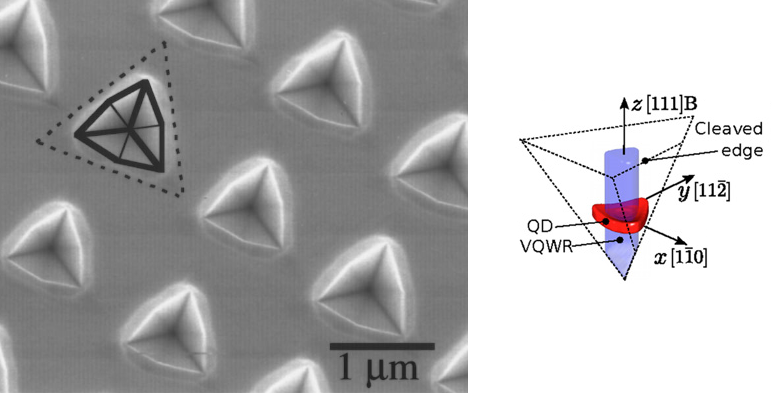
\includegraphics[width=0.8\textwidth]{figures/pyramidal_qds}
 \caption{The tetrahedral recesses within which the QDs are grown. Dashed lines indicate the pyramid boundaries before growth, the solid lines indicate the vicinal facets after growth. ``VQWR'' refers to the vertical quantum wire present in the structure. Recess figure taken from \cite[Fig.~1]{pyramidal_qds}; QD structure diagram taken from \cite[Fig.~1]{karlsson}\label{fig:pyramidal_qds}}
\end{center}
\end{figure}

The quantum dot bulk is an $\text{In}_{0.10}\text{Ga}_{0.90}\text{As}$ alloy semiconductor, and the dot is grown in tetrahedral recesses on a GaAs $\{111\}B$ substrate. Within each tetrahedral recess, three quantum wires form along the pyramid corners, and a quantum dot forms at the tip of the pyramid where the quantum wires meet \cite{pyramidal_qds}. As seen in Fig.~\ref{fig:pyramidal_qds}, the shape of the recess should determine the symmetries of the dot. The triangular base yields the three-fold rotation about the $z$-axis, and the inclination of the facets breaks the $z$-mirror symmetry. However, as seen by the deformation of the facets, the true shape of the dot is affected by several phenomena, some of which are poorly understood.

For instance, Holsgrove \textit{et al.} \cite{hexagon} have studied a similar quantum dot which significantly differs only in the thickness of the lateral quantum wires, and have found the dot to form the shape of a regular hexagon, which does possess $C_{6v}$ symmetry (see Fig.~\ref{fig:hexagonal_qds}). We do not believe that our dot also forms a regular hexagon, and even in such case the true symmetry would be limited by the underlying lattice, hence disconfirming $C_{6v}$ as the group towards which symmetry elevates. However, this illustrates that the true shape of the QD is poorly understood, and might exhibit properties which allow approximate symmetries to manifest.

Dupertuis \textit{et al.} claim that symmetry elevation manifests in strain-free QDs \cite[p.~4]{dupertuis}, and hence we disregard strain effects and symmetry breaking possibly caused by them in our analysis, and we discuss the possible effects of strain on our models in Sec.~\ref{sec:symmetry_outside_gamma} and Sec.~\ref{sec:conclusions}.

\begin{figure}
\begin{center}
    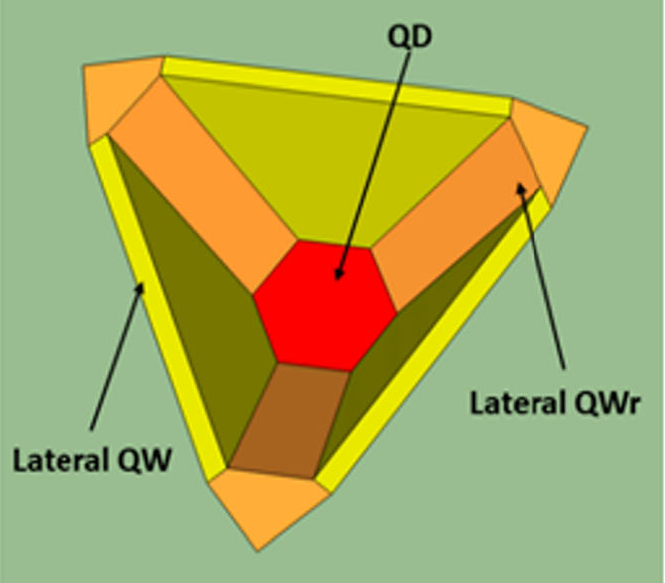
\includegraphics[width=0.4\textwidth]{figures/hexagonal_qds}
 \caption{Analogously-grown QDs form regular hexagons. ``QW'' labels quantum wells, ``QWr'' labels quantum wires. Figure taken from \cite[Fig.~1]{hexagon}\label{fig:hexagonal_qds}}
\end{center}
\end{figure}

The measurements were conducted by our colleagues Francesco Mattana, Luca Colavecchi, Gediminas Juska and Emanuele Pelucchi (Tyndall National Institute, University College Cork). The data will be published together with the experimental details and descriptions of the methods they used to identify emission lines with the exciton transitions they correspond to in a separate paper, and therefore we omit this information here. Mattana, Colavecchi, Juska, and Pelucchi have kindly provided us with the results of their measurements of the spectral features of individual exciton decays, which we use to test our theoretical model in Sec.~\ref{sec:testing_against_data}. 

\pagebreak

\section{Discussions of theory employed}

\subsection{The InGaAs pyramidal quantum dot} \label{sec:growth}
A brief description of the growth process as employed by Karlsson, Pelucchi etc. A discussion of \cite{hexagon} and its arguments for the true shape. A review of effects that alter the shape (and hence the symmetry) of a quantum dot, including strain and other mechanical effects.

\subsection{Exciton complexes and double groups} \label{sec:exciton_theory}
The physical phenomenon which is subject to our study is photoluminiscence. Since this mechanism does not have the QDs in a laboratory ensemble interact or "communicate", we can formulate a theoretical model of photoluminiscence on a singular QD. An external electromagnetic field in the form of a light-beam interacts with the QD in a non-resonant way (as for not to favour a single excited state), which promotes electrons into the conduction band and holes into the valence bands (since there are typically two valence bands at the band edge, which touch at $\Gamma$). The population of excited electrons and different characteristics of holes is called an exciton complex. Exciton complexes decay into lower-occupancy exciton complexes via electron-hole recombination, which produces bright emission lines in the photoluminiscence spectrum. These lines are sharp and occur at fixed frequencies corresponding to the energy level differences, and the theoretical description of their spectrum is the ultimate goal of this work.

Exciton complexes are labelled by the number of electron-hole pairs and the occupancy numbers of each hole type. For example, $2X^+_{21}$ has $2$ electrons, $2$ heavy holes, $1$ light hole, and an overall charge of $+1e$.

In the Karlsson \textit{et al.} system, the light-beam is a laser with a spot size of $\SI{1}{\micro\metre}$, power in the range $25$--$\SI{750}{\nano\watt}$, and wavelength of $\SI{532}{\nano\metre}$. The semiconductor nanocrystal has a direct band-gap at $\Gamma$. The excitons with resolvable emissions have low occupancy numbers (3 or fewer of any of the three fermions--electrons, light holes, and heavy holes). Since the number of fermions excited on a single band is smaller than the number of states available on the band by many orders of magnitude (GIVE ROUGH ESTIMATE), we approximate the exciton complexes as living on $\Gamma$, i.e. each excited fermion having zero crystal momentum.

INSERT BAND STRUCTURE DIAGRAM HERE

Clearly, the phenomenon of photoluminiscence and its behaviour is wholly described by the specific wavefunctions of the exciton complexes. However, finding the wavefunctions and the matrix elements of interaction operators is a near-impossible task and is not viable to make predictions about the spectrum of the quantum dot. However, we can make multiple very strong qualitative predictions (mainly regarding degeneracies of energy levels and selection rules) by using purely symmetry arguments, using the formalism of group theory. To employ group theory, we must first identify the physical symmetries of our quantum dot.

\subsubsection{Envelope function method} \label{sec:envelopes}
The following approach is informed by that developed by Burt (1999), \cite{envelope_fundamentals}. Let us consider a QD with a single excited electron which is promoted to the conduction band (the following easily generalises to holes promoted to valence bands). Disregarding the spin component of its wavefunction for simplicity, we decompose the electron's spatial wavefunction $\Psi\left(\vec{r}\right)$ into plane-waves:
\begin{equation}
\Psi\left(\vec{r}\right)=\int\dd\vec{k} \tilde{\Psi}\left(\vec{k}\right)\exp{i\vec{k}\vdot\vec{r}}
\end{equation}
where $\tilde{\Psi}\left(\vec{k}\right)$ is the Fourier transform of $\Psi\left(\vec{r}\right)$. We now decompose the integral domain into the first Brillouin zone (B.Z.) summed over the set of reciprocal lattice vectors $G$:
\begin{equation}
\Psi\left(\vec{r}\right)=\sum_{\vec{g}\in G}\int_{\vec{k}\in\text{1st B.Z.}}\dd\vec{k} \tilde{\Psi}\left(\vec{k}+\vec{g}\right)\exp{i\left(\vec{k}+\vec{g}\right)\vdot\vec{r}}
\end{equation}
Note that $G$ is equivalent to the set of wave-vectors of plane waves periodic on the Bravais lattice. Therefore, we can choose a set of basis functions $U_n\left(\vec{r}\right)$ periodic on the Bravais lattice like so:
\begin{eqnarray}
U_n\left(\vec{r}\right)&=&\sum_{\vec{g}\in G}u_{n}\left(\vec{g}\right)\exp{i\vec{g}\vdot\vec{r}}\\
U_n\left(\vec{r}+\vec{r}_B\right)&=&\sum_{\vec{g}\in G}u_{n}\left(\vec{g}\right)\exp{i\vec{g}\vdot\vec{r}}\exp{i\vec{g}\vdot\vec{r}_B}=U_n\left(\vec{r}\right)
\end{eqnarray}
where $\vec{r}_B\in R$ is a lattice vector and $u_n\left(\vec{g}\right)$ are the coefficients of the decomposition of $U_n$ into reciprocal lattice plane waves, typically chosen such that $U_n$ are orthonormal. Then, inverting this decomposition, we obtain
\begin{equation}
\exp{i\vec{g}\vdot r} = \sum_n u_n\left(\vec{g}\right)^*U_n\left(\vec{r}\right)
\end{equation}
which allows us to decompose the original wavefunction into a sum of the orthonormal basis vectors $U_n$ and their envelope functions $\Upsilon_n$:
\begin{eqnarray}
\Psi\left(\vec{r}\right)&=&\sum_n \Upsilon_n\left(\vec{r}\right)U_n\left(\vec{r}\right)\\
\Upsilon_n\left(\vec{r}\right)&=&\sum_{\vec{g}\in G}\int_{\vec{k}\in\text{B.Z.}}\dd\vec{k}u_n\left(\vec{g}\right)^*\tilde{\Psi}\left(\vec{k}+\vec{g}\right)\exp{i\vec{k}\vdot\vec{r}}
\end{eqnarray}
Now, we choose $U_n\left(\vec{r}\right)$ to represent the band-edge wavestates in the bulk structure. Using a tight-binding model with spin-orbit coupling, these wavestates can be labelled by three quantum numbers: total angular momentum $j$, its projection onto the $z$-axis $j_z$, and the orbital energy excitation $\varepsilon_n$, which we assume to be in the ground state in our system due to energy occupancy statistics (as we expect the population of states other than in the ground state to be negligible for a low-power light-source). Furthermore, the quantum number $j$ is determined by the orbital angular momentum $l$, which is given by the electron configuration in each specific band, and the spin $s=1/2$ determined for electrons and electron holes by their fundamental properties.

Photonic nanostructures can, on a small scale, cease to posses a standard band-structure, instead featuring e.g. flat bands. Dresselhaus \textit{et al.} (2007) quotes the number of Bravais lattice cells below which this occurs to be in the order of $10^2$ \cite[p. 213]{dresselhaus_condensed_matter}. Our QDs have volumes typically higher than $\SI{100}{\nano\metre\cubed}$ \cite[p. 2]{karlsson_2010}, which corresponds to the number of unit cells in the order of $10^3$. Hence we can reasonably expect our system to posses a band structure. This has two consequences to our envelope function model:
\begin{enumerate}
\item The envelope function $\Upsilon\left(\vec{r}\right)$ is varying slowly enough for it to have an approximately defined crystal momentum. As discussed in \ref{sec:exciton_theory}, we assume $k\approx 0$.
\item The wavefunction $\Psi\left(\vec{r}\right)$ of a single excited fermion approximately corresponds to a single state on the excited band of the infinite bulk crystal band structure. In other words, there exists a basis vector $U_n$ such that for all other basis vectors $U_m, m\neq n$, their contribution to the wavefunction is negligible.
\end{enumerate}
Labelling the single contributing basis vector by the quantum numbers $l, s, j, j_z$, we can express the wavefunction of a single excited fermion as
\begin{equation}
\braket{\vec{r}}{\Psi}=\Upsilon\left(\vec{r}\right)\braket{\vec{r}}{l, s=1/2, j, j_z}
\end{equation}
As discussed in Burt (1992) \cite[p. 6656]{envelope_equation}, we can write down the effective Hamiltonian for the envelope function, which yields the corresponding Schrödinger equation:
\begin{eqnarray}
\hat{H}_\Upsilon &=& -\frac{\hbar^2}{2}\nabla\vdot\frac{1}{m^*\left(\vec{r}\right)}\nabla + E_0\\
\hat{H}_\Upsilon \Upsilon\left(\vec{r}\right)&=& E\Upsilon\left(\vec{r}\right)
\end{eqnarray}
where $E_0$ is the band-edge energy. Now, in a parabolic Taylor expansion of the bands about $\Gamma$, we state that around the $\Gamma$ point the effective mass $m^*$ is constant. We now see that the Schrödinger equation reduces to the following form:
\begin{equation}\label{eq:single_envelope_function}
-\frac{\hbar^2}{2m^*}\nabla^2 \Upsilon = (E-E_0)\Upsilon
\end{equation}
This is the equation of a free particle with energy $E_p=E-E_0$. Hence we can model a single excited fermion as a "particle in a box" around the $\Gamma$ point for a large enough structure.

Now we consider the wavefunction of an exciton complex, which is comprised of multiple excited fermions. The interaction between the fermions is purely electromagnetic. Since the envelope functions are slowly-varying and associated to zero crystal momenta, their magnetic interaction is negligible. The magnetic interaction of the periodic basis functions gives rise to spin-orbit and orbit-orbit coupling (ignoring the hyperfine structure of spin-spin coupling), which allows us to label an exciton complex with a total angular momentum $J$ and its projection onto the $z$-axis $J_z$ as two quantum numbers. The Coulomb interaction between fermions $a$ and $b$ gives rise to a term in the Hamiltonian in the form
\begin{equation}
\hat{V}_{ab}^C\left(\vec{r}_a,\vec{r}_b\right)=\frac{q_aq_b}{4\pi\epsilon_0}\frac{1}{\abs{\vec{r}_a-\vec{r}_b}}
\end{equation}
This operator can be rewritten as a function of a single vector:
\begin{equation}
\hat{V}_{ab}^C\left(\vec{\xi}\right)=\frac{q_aq_b}{4\pi\epsilon_0}\frac{1}{\xi}, \qq{} \xi = \abs{\vec{\xi}}
\end{equation}
Note that when this operator acts on the full two-particle wavefunction:
\begin{equation} \label{eq:coulomb_interaction_integral}
\hat{V}_{ab}^C\left(\vec{r}_a-\vec{r}_b\right)\Upsilon_a\left(\vec{r}_a\right)U_a\left(\vec{r}_a\right)\Upsilon_b\left(\vec{r}_b\right)U_b\left(\vec{r}_b\right)
\end{equation}
the envelope functions $\Upsilon_a, \Upsilon_b$ are slowly-varying, so we can state that they don't change in the volume of a single crystal lattice cell. Therefore, we can take the envelope functions outside of an integral where each vector $\vec{r}_a, \vec{r}_b$ is confined to a single cell:
\begin{eqnarray*}
\int_{\vec{r}_a\in \text{cell a}}\dd^3 \vec{r}_a \int_{\vec{r}_b\in \text{cell b}} \dd^3 \vec{r}_b \hat{V}_{ab}^C\left(\vec{r}_a-\vec{r}_b\right)\Upsilon_a\left(\vec{r}_a\right)U_a\left(\vec{r}_a\right)\Upsilon_b\left(\vec{r}_b\right)U_b\left(\vec{r}_b\right) \approx \\
\Upsilon_a\left(\vec{r}_a\right)\Upsilon_b\left(\vec{r}_b\right) \int_{\vec{r}_a\in \text{cell a}}\dd^3 \vec{r}_a \int_{\vec{r}_b\in \text{cell b}} \dd^3 \vec{r}_b \hat{V}_{ab}^C\left(\vec{r}_a-\vec{r}_b\right)U_a\left(\vec{r}_a\right)U_b\left(\vec{r}_b\right)
\end{eqnarray*}
and since $U_a, U_b$ are periodic over the crystal lattice, we can denote $\xi = \vec{R}_{\text{cell b}}-\vec{R}_{\text{cell a}}$ to be the lattice vector equal to the displacement between the two cells, then the integral becomes
\begin{eqnarray*}
\int_{\vec{r}_a\in \text{cell a}}\dd^3 \vec{r}_a \int_{\vec{r}_b\in \text{cell b}} \dd^3 \vec{r}_b \hat{V}_{ab}^C\left(\vec{r}_a-\vec{r}_b\right)\Upsilon_a\left(\vec{r}_a\right)U_a\left(\vec{r}_a\right)\Upsilon_b\left(\vec{r}_b\right)U_b\left(\vec{r}_b\right) \approx \\
\Upsilon_a\left(\vec{r}_a\right)\Upsilon_b\left(\vec{r}_b\right) \int_{\vec{r}_a\in \text{U.C.}}\dd^3 \vec{r}_a \int_{\vec{r}_b\in \text{U.C.}} \dd^3 \vec{r}_b \hat{V}_{ab}^C\left(\vec{r}_a-\vec{r}_b-\vec{\xi}\right)U_a\left(\vec{r}_a\right)U_b\left(\vec{r}_b\right)
\end{eqnarray*}
where U.C. denotes a single unit cell of the crystal lattice centered around the origin (or otherwise fixed in space). Now comes the final approximation. When considering the integral of the expression \ref{eq:coulomb_interaction_integral} over an arbitrary dual volume, we partition the volumes into unit cells of the crystal lattice and then divide the integral into pairwise U.C.-U.C. integrals over a set of displacement vectors $\vec{\xi}$. For the majority of these vectors in dual volumes comparable in size to the size of the QD, the values of $\xi$ will be larger than the dimensions of U.C. Hence we can approximate
\begin{equation}
\hat{V}_{ab}^C\left(\vec{r}_a-\vec{r}_b-\vec{\xi}\right)\approx \hat{V}_{ab}^C\left(\vec{\xi}\right)
\end{equation}
By denoting the set of lattice vectors in the volume $V$ as $R_V$, the integral simplifies to
\begin{eqnarray*}
\int_{V}\dd^3 \vec{r}_a\int_{V}\dd^3 \vec{r}_b \hat{V}_{ab}^C\left(\vec{r}_a-\vec{r}_b\right)\Upsilon_a\left(\vec{r}_a\right)U_a\left(\vec{r}_a\right)\Upsilon_b\left(\vec{r}_b\right)U_b\left(\vec{r}_b\right) \approx \\
\Pi_{ab} \sum_{\vec{r}_a\in R_V}\sum_{\vec{r}_b\in R_V} \hat{V}_{ab}^C\left(\vec{r}_a-\vec{r}_b\right)\Upsilon_a\left(\vec{r}_a\right)\Upsilon_b\left(\vec{r}_b\right)\\
\qq{where}\Pi_{ab} = \int_{\vec{r}_a\in \text{U.C.}}\dd^3 \vec{r}_a \int_{\vec{r}_b\in \text{U.C.}} \dd^3 \vec{r}_b U_a\left(\vec{r}_a\right)U_b\left(\vec{r}_b\right) \qq{is a correlation constant.}
\end{eqnarray*}
Now we renormalize the correlation constant $\Pi_{ab}$ using the volume of the unit cell $V_{\text{U.C.}}$, which allows us to rewrite the double sum over $R_V$ as an integral over the dual volume:
\begin{eqnarray*}
\int_{V}\dd^3 \vec{r}_a\int_{V}\dd^3 \vec{r}_b \hat{V}_{ab}^C\left(\vec{r}_a-\vec{r}_b\right)\Upsilon_a\left(\vec{r}_a\right)U_a\left(\vec{r}_a\right)\Upsilon_b\left(\vec{r}_b\right)U_b\left(\vec{r}_b\right) \approx\\
 \Pi'_{ab} \int_{V}\dd^3 \vec{r}_a\int_{V}\dd^3 \vec{r}_b  \hat{V}_{ab}^C\left(\vec{r}_a-\vec{r}_b\right)\Upsilon_a\left(\vec{r}_a\right)\Upsilon_b\left(\vec{r}_b\right),\\
 \qq{where} \Pi'_{ab}=V_{\text{U.C.}}^{-2}\Pi_{ab}=\langle U_a\left(\vec{r}_a\right)U_b\left(\vec{r}_b\right)\rangle_{\text{U.C.}}
 \end{eqnarray*}
 Since this must be true for any (sufficiently large) $V$, we drop the integral altogether, equating the integrands:
 \begin{equation}
 \hat{V}_{ab}^C\left(\vec{r}_a-\vec{r}_b\right) \Psi_a\left(\vec{r}_a\right)\Psi_b\left(\vec{r}_b\right) = \Pi'_{ab}\hat{V}_{ab}^C\left(\vec{r}_a-\vec{r}_b\right)\Upsilon_a\left(\vec{r}_a\right)\Upsilon_b\left(\vec{r}_b\right)\qq{on vol. avg.}
 \end{equation}
 What was done here was essentialy taking a volume average over the product of the basis functions $U_aU_b$, motivated by their periodicity over unit volumes much smaller than that of the quantum dot. This high-frequency periodicity manifests as a simple correlation coefficient when considering matrix elements of $\hat{V}_{ab}^C$.
 
 This allows us to modify \ref{eq:single_envelope_function} to account for Coulomb interaction purely in the paradigm of envelope functions. The full effective Schrödinger equation for envelope functions (since the fine structure effects do not matter for the slowly-varying envelope functions) is then
 \begin{equation} \label{eq:exciton_envelope_equation}
 \left(-\sum_{i}\frac{\hbar^2}{2m_i^*}\nabla_{\vec{r}_i}^2 +\sum_{i,j; i\neq j} \Pi'_{ij}\hat{V}_{ij}^C\left(\vec{r}_i-\vec{r}_j\right) \right)\Upsilon = E_{\text{exciton}}\Upsilon
 \end{equation}
 where
 \begin{equation*}
 \Upsilon = \prod_{i}\Upsilon_i\left(\vec{r}_i\right)
 \end{equation*}
 Note that the Coulomb interaction on the volumes of the scale of the unit cell of the crystal lattice is fully rotationally symmetric, and therefore will not invalidate $J, J_z$ as good quantum numbers. However, it will affect the value of $\Pi'_{ij}$, which therefore becomes nontrivial to calculate. It will also affect the shape of the periodic functions, which we can for simplicity just denote $F_i\left(\vec{r}_i\right)$, and which have the same periodic properties as $U_i\left(\vec{r}_i\right)$, and form in totality a $J, J_z$ eigenstate. Therefore, we expect the transformation $U_i\to F_i$ to only affect the radial dependence in the close vicinity of an atom, preserving the spherical-harmonics angular dependence in the tight-binding model.
 
 By interpreting eq. \ref{eq:exciton_envelope_equation}, we now see that the envelope functions in an exciton complex behave as free particles in a box with added Coulomb interactions, i.e. a many-body charged particle system. Note that the potential barriers at the edges of the "box" are not infinite, and that would indeed not be a good approximation!
 
 \textit{Note.} Even though $\hat{V}_{ab}^C\left(\vec{r}_a-\vec{r}_b\right)$ diverges for $\vec{r}_a=\vec{r}_b$ (which occurs in the small subset of $R_V\otimes R_V$ where both vectors are in the same unit cell), the contribution of the integrals over these coinciding unit cells should not be disproportionally high, since when considering the volume integral in spherical coordinates centered on the asymptote, the integrand goes like $\abs{\vec{r}_a-\vec{r}_b}$, so the integral should be approximately proportional to $V_{\text{U.C.}}^{2/3}$, and the contribution from this subset where our approximations fail to the total integral is negligible.

\subsubsection{Symmetry arguments, group theory, and double groups} \label{sec:symmetry_arguments}
Now that we have decomposed the single excited fermion wavefunction into a $j$-eigenstate periodic in the atomic lattice and a slowly varying envelope function which corresponds to a zero bulk-crystal momentum, we turn to symmetry arguments to make predictions about the spectrum. Indeed, finding either of the two component functions is a task beyond the scope of this work, but we can make quantitative statements about the splitting of the exciton energy levels and selection rules for transitions between these energy levels. To do this, we must consider how the exciton wavefunction transforms under symmetry transformations of the true Hamiltonian.

To review the basic applications of group theory to quantum mechanics as outlined e.g. in Dresselhaus (2002) \cite{dresselhaus}, we consider the set of rotations commuting with a Hamiltonian $\hat{H}$. This set forms a group under multiplication (as for $\hat{R}_1, \hat{R}_2$ commuting with $\hat{H}$, $\hat{R}_1\hat{R}_2$ must be a single rotation $\hat{R}_3$ which also commutes with $\hat{H}$). This group shall be denoted as $G_{\hat{H}}$, and is referred to as the group of the Hamiltonian. As shown in standard texts, each energy level $E_n$ of the time-independent Schrödinger eigenvalue problem $\hat{H}\Psi_n=E_n\Psi_n$ corresponds to an irreducible representation (irrep) of $G_{\hat{H}}$, which we can denote as $\Gamma_{r(n)}$, where $r$ is some mapping. The degeneracy of $E_n$ is then equal to the dimension of $\Gamma_{r(n)}$. Therefore, knowing the group of the Hamiltonian tells us the possible degeneracies of the energy levels and what they transform like under the symmetry transformations.

Moreover, group theory has an application to selection rules. Consider two energy levels $E_a, E_b$ of a system with the Hamiltonian $\hat{H}$. If we add a perturbation $\hat{H}'$ which allows transition between energy levels, and which transforms according to the representation $\Gamma_{\hat{H}'}$, by Fermi's golden rule the rate of transition $E_a\to E_b$ is proportional to the matrix element $\mel{E_a}{\hat{H}'}{E_b}$ (if the energy levels are degenerate, we need to pick a set of basis vectors and consider the rates of transition between each pair of basis vectors). As per \cite[Ch. 7]{dresselhaus}, this matrix element vanishes if the irrep direct product $\Gamma_{r(a)}\otimes\Gamma_{\hat{H}'}\otimes\Gamma_{r(b)}$ does not contain the identity representation. This allows us to decide which exciton transitions under photoluminiscent electron-hole recombination will be dark in which polarisation.

Consider now the effective Hamiltonians acting on the envelope function $\Upsilon=\prod_{i}\Upsilon_i\left(\vec{r}_i\right)$ and the 
periodic function $F=\prod_{i}F_i\left(\vec{r}_i\right)$, respectively.
\begin{enumerate}
\item $\Upsilon$, representing a many-body charged particle-in-a-box system, is governed in its symmetry by the shape of the box, i.e. the shape of the QD. In our system, this shape is assumed to posses $C_{3v}$ (tetrahedral) symmetry. This symmetry shall be referred to as the \textit{structure symmetry}.
\item $F$, representing a function periodic in the crystal lattice, is governed in its symmetry by the shape of the lattice, i.e. the properties of the bulk of the crystal. In our system, the crystal lattice is a zincblend structure (cubic FCC) around the [111] direction. The point group of this lattice is $T_d$. This symmetry shall be referred to as the \textit{bulk symmetry}.
\item Around the individual atoms in the crystal lattice, in the tight-binding model the exciton forms a total angular momentum eigenstate $\ket{J, J_z}$. This has a full roto-inversion symmetry, and since it is a spin-half spinor, the group describing the full roto-inversion symmetry is $SU(2)\otimes C_i$, where $C_i=\{\hat{E}, \hat{i}\}$ is the inversion group and it is isomorphic to $\mathbb{Z}_2$.
\end{enumerate}
Naturally, the symmetry of the true Hamiltonian will be the lowest one of these, which is in our case the structure symmetry $C_{3v}$--or rather, since we are discussing spin-half spinors, its double group, as will be discussed below. However, as we argue below, the bulk symmetry will be important when explaining the origin of symmetry elevation in our perturbative model.

Now, let us consider the character of the full exciton wavefunction under a symmetry transformation $\hat{R}$. Since the Coulomb interaction transforms according to the identity rep under roto-inversions, we can first consider the character of a single fermion wavefunction under the symmetry transformation, and then we construct the full exciton character through $j$-coupling, as discussed in Sec. \ref{sec:j_coupling}. Since the single excited fermion wavefunction is a product of two functions, its character will be the product of the two constituent characters:
\begin{equation} \label{eq:character_breakdown}
\chi^{\left(\Psi\left(\vec{r}\right)\right)}\left(\hat{R}\right)=\chi^{\left(\Upsilon\left(\vec{r}\right)\right)}\left(\hat{R}\right)\chi^{\left(U\left(\vec{r}\right)\right)}\left(\hat{R}\right)
\end{equation}
The character of the envelope function can be, in principle, any irrep of the structure symmetry group. However, we once again invoke the energy statistics--the population of QDs excited by a low-energy laser for which the envelope functions are out of the ground state should be negligible. Therefore, assuming the envelope function is in its ground state, we know it transforms according to the identity rep. Therefore $\chi^{\left(\Upsilon\left(\vec{r}\right)\right)}\left(\hat{R}\right)=1$.

In the tight-binding model, the band-edge eigenstate $U$ is a convolution of the $j$-eigenstate which exists around each atom with the distribution of the atoms, weighted relatively to their atomic properties. Since the structure symmetry group is a subgroup of the bulk symmetry group, the bulk crystal lattice maps onto itself under every rotation in the structure symmetry. Furthermore, the Ga-As bonds in the conduction band are antisymmetric, and the second-nearest neighbour bonds are symmetric \cite{gaas_bonding}, which leaves the lattice to transform according to the identity rep. (FIGURE HERE)

Therefore the only part of the single excited fermion wavefunction which does not necessarily transform according to the identity rep is the $j$-eigenstate itself. The character of a $j$-eigenstate is just the trace of the corresponding Wigner D-matrix (CITATION), and each set of eigenstates
\begin{equation*}
\mqty(\ket{j,j_z=j}\\\ket{j,j_z=j-1}\\\vdots\\\ket{j, j_z=-j})\mbox{ forms a basis to }\Gamma^{(SU(2))}_{j}
\end{equation*}
To extend this unto roto-inversions, we need to consider the orbital angular momentum $l$, which determines inversion parity. For example, in our system, the conduction band is an $s$-orbital, which has even parity under inversion, but the valence band is a $p$-orbital, which has odd parity under inversion. Determining parity specifies the irrep of the full roto-inversion group $SU(2)\otimes C_i$, which gains an index $g$ (gerade) if even or $u$ (ungerade) if odd under inversion.

Our approach to construct the transformation laws for the single excited fermions is therefore to consider the irreps of the full roto-inversion spinor group, and then decompose them into the true symmetry, i.e. the structure symmetry. To do this, we must construct the double group of the structure symmetry point group. Essentially, a double group encodes the spin-orbit coupling for its original group by adding the time-reversal operator as a generator. This renders rotations by $2\pi$ to result in time-reversal, and only rotations by $4\pi$ return back to the identity, in agreement with the behaviour of spin-half particles under rotation. The theory of double groups is outlined in \cite[Ch. 19]{dresselhaus}, and the character tables of double groups can be found in standard tables, such as \cite{altmann}.

Applying this approach, we find that an electron promoted to the $s$-orbital conduction band transforms according to $\Gamma_{j=1/2, g}$ in the full roto-inversion group, which reduces to $E_{1/2}$ in the $C_{3v}$ double group. Conversely, a hole promoted to the $p$-orbital valence band transforms according to $\Gamma_{j=1/2, u}\oplus\Gamma_{j=3/2, u}$ in the full roto-inversion group. We identify $\Gamma_{j=1/2, u}$ as the split-off band which has lower energy at the band-edge, and hence will not be populated in our system. Conversely, $\Gamma_{j=3/2, u}$ decomposes into $E_{1/2}\oplus E_{3/2}$ in the $C_{3v}$ double group, where $E_{1/2}$ corresponds to the light-hole band ($j_z=\pm 1/2$) and $E_{3/2}$ corresponds to the heavy-hole band ($j_z=\pm 3/2$). This also illustrates the symmetry-informed reason why there are two different hole types.

\subsubsection{Total angular momentum coupling and Pauli's exclusion principle} \label{sec:j_coupling}
To obtain the transformation properties of an exciton complex, we must consider the magnetic orbit-orbit and spin-orbit interaction which couples the total angular momenta $j$ of separate fermions together. The treatment of $j$-coupling in the full roto-inversion symmetry is as follows:

Consider two non-interacting particles governed by Hamiltonians which conserve total angular momentum. Let the two particles exist in $j$-eigenstates $\ket{j^A, j^A_z, p}, \ket{j^B, j^B_z, p}$ respectively (here $p$ specifies the inversion parity), and the group of each of their Hamiltonians is $SU(2)\otimes C_i$. The full Hilbert space they occupy is the direct product of the Hilbert space occupied by each particle, and hence the group of the total Hamiltonian is:
\begin{equation}
G^{\text{nonint.}}_{\hat{H}}=\left(SU(2)\otimes C_i\right)\otimes\left(SU(2)\otimes C_i\right)
\end{equation}
The irreps of this group are the direct products of the respective irreps $\Gamma_{j,p}$, and hence
\begin{equation} \label{eq:noninteracting_j}
\ket{j^A, j^A_z, p^A}\otimes\ket{j^B, j^B_z, p^B}\qq{transforms according to}\Gamma_{j^A, p^A}\otimes\Gamma_{j^B, p^B}
\end{equation}
If we now include an interaction term in the full Hamiltonian which couples the total angular momenta of the particles, $j^A_z, j^B_z$ cease to be good quantum numbers. Instead (in classic electromagnetic coupling), the full total angular momentum $J$ and its projection along the $z$-axis, $J_z$, become good quantum numbers. Preserving $j^A, j^B$ as immutable parameters of the physical system, the new energy eigenstates posses the roto-inversion symmetry $SU(2)\otimes C_i$, and transform according to its irreps--this is determined wholly by the quantum numbers, which specify the partitioning of the Hilbert space into degenerate subspaces. Hence we need to reduce the high-symmetry irrep in Eq. \ref{eq:noninteracting_j} into the lower-symmetry group $SU(2)\otimes C_i$.

A decomposition is always unique by the Great Orthogonality Theorem (CITATION), therefore finding a decomposition is sufficient to prove it is the correct one. We will assume that all constituent irreps in the decomposition have equal parity, which is the product of the two parities $p^A\cdot p^B$. Then, using standard results (CITATION), we write down the decomposition:
\begin{equation}
\Gamma_{j^A, p^A}\otimes\Gamma_{j^B, p^B}=\sum_{J=\abs{j^A-j^B}}^{j^A+j^B}\Gamma_{J, p^A\cdot p^B}
\end{equation}
We can now generalise this approach to cases where each particle's original Hamiltonian undergoeas symmetry breaking to some double group $\tilde{G}_{\hat{H}_0}$, which is a subgroup of $SU(2)\otimes C_i$. In the non-interacting direct product of the two Hilbert spaces, each pair of quantum numbers $j^i, j^i_z$ reduces into an instance of this subgroup, and so the pair of non-interacting particles transforms according to $\tilde{G}_{\hat{H}_0}\otimes\tilde{G}_{\hat{H}_0}$. If we include the $j$-coupling interaction term, the full system features only one pair of these quantum numbers, $J, J_z$, which reduce into a single instance of the aforementioned subgroup. Hence, the reduction goes like this:
\begin{equation}
\Gamma^{\left(\tilde{G}_{\hat{H}_0}\right)}_A \otimes \Gamma^{\left(\tilde{G}_{\hat{H}_0}\right)}_B \to \bigoplus_i \Gamma^{\left(\tilde{G}_{\hat{H}_0}\right)}_i
\end{equation}
Naturally, as the constituent irreps in the direct sum on the right side correspond to different energy levels (disregarding accidental degeneracy), the symmetry breaking associated with coupling of quantum numbers lowers the degeneracy of the system.

The outlined method is sufficient for finding the energy levels of distinguishable particles undergoing coupling; however, in our case, the particles are fermions, and hence, for particles occupying the same $k$-state in the same band, we also have to consider Pauli's exclusion principle.

The conduction band is an $s$-orbital, and hence the excited electrons have $j=1/2$, which renders their $k$-states doubly degenerate. The valence band is a $p$-orbital, and hence the holes have $j=3/2$ and $4$-fold degenerate $k$-states. However, for most groups, including $C_{3v}$, the $SU(2)\otimes C_i$ irrep $\Gamma_{j=3/2,u}$ reduces to two $2$-dimensional irreps, which causes the holes to have two different characters (light-like and heavy-like), each with doubly degenerate $k$-states. We assume that the bands fill up sequentially under excitation in a way that maximises the number of completely filled-out states.
\begin{itemize}
\item For doubly degenerate $k$-states, we only need to find the transformation properties of the full $k$-state, i.e. a pair of fermions. As per Karlsson \textit{et al.} \cite[p. 15]{karlsson}, a full doubly degenerate energy level transforms according to the identity representation.
\item For $4$-fold degenerate $k$-states with $j=3/2$, we can extend Karlsson's argument to claim that the full energy level with $4$ particles transforms according to the identity representation. We can label an energy level with $3$ particles by the $1$ missing particle, and hence it transforms equally to an energy level filled with $1$ particle. Finally, for two particles, we need to construct the $6$ antisymmetric basis vectors, with kets labelled by the $j_z$ values of the first and the second particle respectively:

\begin{center}
\begin{tabular}{ll}
$b_1=\frac{1}{\sqrt{2}}\left(\ket{\frac{3}{2},-\frac{3}{2}}-\ket{-\frac{3}{2},\frac{3}{2}}\right)$ & $b_2=\frac{1}{\sqrt{2}}\left(\ket{\frac{1}{2},-\frac{1}{2}}-\ket{-\frac{1}{2},\frac{1}{2}}\right)$ \vspace{0.2cm}\\
$b_3=\frac{1}{\sqrt{2}}\left(\ket{\frac{3}{2},\frac{1}{2}}-\ket{\frac{1}{2},\frac{3}{2}}\right)$ & $b_4=\frac{1}{\sqrt{2}}\left(\ket{-\frac{3}{2},-\frac{1}{2}}-\ket{-\frac{1}{2},-\frac{3}{2}}\right)$ \vspace{0.2cm}\\
$b_5=\frac{1}{\sqrt{2}}\left(\ket{\frac{3}{2},-\frac{1}{2}}-\ket{-\frac{1}{2},\frac{3}{2}}\right)$ & $b_6=\frac{1}{\sqrt{2}}\left(\ket{-\frac{3}{2},\frac{1}{2}}-\ket{\frac{1}{2},-\frac{3}{2}}\right)$
\end{tabular}
\end{center}

The character of a rotation is given purely by the angle $\theta$, not by the rotation axis, as
\begin{equation} \label{eq:weyl_character}
\chi^{\left(\Gamma_{j}\right)\left(\hat{R}(\theta)\right)}=\frac{\sin{\left(2j+1\right)\theta/2}}{\sin{\theta/2}}
\end{equation}
which is just the trace of the Wigner $d$-matrix, which Wigner defined as
\begin{equation}
d^j_{m',m}=\mel{j,m'}{\hat{R}(\theta)}{j,m}
\end{equation}
where $\theta$ is the second Euler angle in the z-y-z convention \cite[p.160]{wigner}, and for which Wigner gave an expression \cite[p.167]{wigner}. The character of a simultaneous rotation of two particles is a product of the two single-particle rotation characters, which allows us to calculate the sum of the simultaneous-rotation characters over all basis vectors:
\begin{equation}
\sum_{i=1}^6 \chi^{b_i}\left(\hat{R}(\theta)\right)=2\cos{\theta}+2\cos{2\theta}+2
\end{equation}
which we can equate to the sum of the characters of $\Gamma_{j=0}\oplus \Gamma_{j=2}$, as per eq. \ref{eq:weyl_character}. Hence an energy level with $j=3/2$ filled with two particles transforms as $\Gamma_{j=0}\oplus \Gamma_{j=2}$.


\end{itemize}

Hence we can label any exciton complex for groups which have one or two hole characters by labelling each fermion type by the number of free fermions and then multiplying the corresponding representations for each fermion type. Reducing this into the irreps of the structure symmetry group gives is the number of energy levels and their degeneracies for each exciton complex.

\subsection{Photoluminiscence spectrum and evidence of symmetry elevation}

To predict the rate of photoluminiscent transitions between energy levels, we utilize the dipole approximation, in which the dipole operator (and hence the perturbing Hamiltonian) transforms as a vector \cite[p. 13]{karlsson}. Vectors transform according to the Cartesian representation, which can be easily constructed from rotation matrices \cite[p. 160]{wigner}. If the Cartesian representation is reducible in the structure symmetry group, different vector orientations of the dipole may transform differently, resulting in different lines in polarised spectra. In that case, we must apply the selection rules outlined in Sec. \ref{sec:symmetry_arguments} for each polarisation separately. Then, the number of allowed transitions between different finely-split energy levels of two excitons gives the number of tightly-spaced lines we predict on the spectrum of that exciton transition.

In \cite{karlsson}, Karlsson \textit{et al.} have applied the selection rules to different exciton transitions and compared the predicted number of lines to their experimental data. (FIGURE HERE) The predictions have mostly agreed, but three exciton transitions were identified for which emission lines in the measured spectra were missing. These were:
\begin{enumerate}
\item $X_{10}\to $vacuum ($2$ predicted $x-y$-polarised lines, $1$ measured).
\item $2X_{20}\to X_{10}$ ($2$ predicted $x-y$-polarised lines, $1$ measured).
\item $2X_{11}\to X_{01}$ ($6$ predicted $x-y$-polarised lines, $3$ resolved strongly and $2$ more resolved weakly).
\end{enumerate}
Karlsson \textit{et al.} theorise that the missing lines or the relative intensity of lines in these transitions can be explained by a symmetry elevation to a larger group of symmetries which contains $C_{3v}$. In our work, we have attempted to test this claim.





\section{Results--symmetry suppression theory}

%\subsection{Treatment of parity}
%The theoretical treatment of parity under $l$ and $j$-coupling is shown. The program AReTDoG as an implementation of this and its agreement with \cite{karlsson} is discussed.

%\subsection{Symmetry suppression theory} \label{sec:suppression}
%The first-order perturbation treatment of selection rules and its applicability to low-to-high symmetry systems is shown.

In our research, we tested the following hypothesis: \textit{Symmetry elevation effects are caused by transformation properties of the bulk symmetry.} Since the bulk symmetry group $T_d$ contains the structure symmetry $C_{3v}$ as a subgroup, it is a natural suspect for a source  of \textit{approximate} symmetries, since it limits the true symmetry of the system.

The theoretical basis for particular excitons enjoying symmetry transformations from the bulk symmetry is built on their localisation within the QD. If the envelope functions $\Upsilon_i$ of every fermion in an exciton complex are localised near the centre of the QD, any bulk-symmetry transformation should also be a symmetry transformation of the exciton wavefunction. With every QD border the envelope functions approach, more approximate symmetry transformations vanish, until, when an exciton has significant probability to measure one or more of its fermions around the entire edge of the QD, it fully probes the structure symmetry.

\subsection{Perturbative analysis of selection rules}
Suppose now we have a system described by a Hamiltonian $\hat{H}$ equipped with a group of symmetries $G$. Let us construct a Hamiltonian $\hat{H}_+$ which is equipped with a group of symmetries $G_+$ such that $G<G_+$ and $\hat{H}$ can be modelled as a perturbation of $\hat{H}_+$ like so:
	$$\hat{H}=\hat{H}_+ + \lambda \hat{H}',\qq{where}\lambda\ll 1$$
	For an exciton with its wavefunction localised in the centre of the QD, $\hat{H}$ is the true Hamiltonian, and $\hat{H}_+$ is the Hamiltonian of a smaller QD inscribed into the true QD with a higher symmetry.
	\subsubsection{Elevated symmetry component of an energy eigenstate}
	Let us denote the eigenstates of the Hamiltonians $\hat{H},\hat{H}_+$ as $\ket{E_i;n}$ and $\ket{E^+_{i'};n'}$ respectively, where $n, n'$ are the degeneracy labels. Disregarding accidental degeneracy, we know that every set of degenerate energy levels forms a basis of (i.e. transforms according to) an irrep of the respective symmetry group:
	$$\mqty(\ket{E_i;1}\\\ket{E_i;2}\\\vdots\\\ket{E_i;d_i})\mbox{ forms a basis to }\Gamma^{(G)}_{r(i)}; \mqty(\ket{E^+_{i'};1}\\\ket{E^+_{i'};2}\\\vdots\\\ket{E^+_{i'};d^+_{i'}})\mbox{ forms a basis to }\Gamma^{\left(G_+\right)}_{r^+(i')}$$
	where $d_i, d^+_{i'}$ specify the total degeneracies of the energy levels and $r,r^+$ are some functions which map energy levels onto irreps.
	Under a first-order perturbation of a set of degenerate eigenstates, the distance of the new states from the subspace $\mathcal{D}^+$ spanned by the degenerate eigenstates goes like $O(\lambda)$. Therefore, if $\ket{E_i;n}$ arises from perturbing a degenerate subspace of energy $E^+_j$, there exists an unnormalized vector $\ket{E^+_j;P}\in\mathcal{D}^+_j$ for which
	\begin{eqnarray*}
	\frac{\braket{E_i;n}{E^+_j;P}}{\abs{\braket{E^+_j;P}{E^+_j;P}}^{1/2}}&=&1-O(\lambda)\\
	\qq{where} \braket{E^+_j;P'}{E_i;n}&=&\braket{E^+_j;P'}{E^+_j;P}
	\qq{for all} \ket{E^+_j;P'}\in\mathcal{D}^+
	\end{eqnarray*}
	We can construct a state satisfying these conditions by projecting the perturbed eigenstate onto the original degenerate subspace:
	\begin{eqnarray*}
	\hat{P}^+_j&=&\sum_{m=1}^{d^+_j}\dyad{E^+_j;m}{E^+_j;m}\\
	\ket{E^+_j;P}&=&\hat{P}^+_j\ket{E_i;n}=\sum_{m=1}^{d^+_j}\ket{E^+_j;m}\braket{E^+_j;m}{E_i;n}
	\end{eqnarray*}
	Now we can express a general eigenstate of $\hat{H}$ as a superposition of an eigenstate of $\hat{H}^+$ with a norm that goes like $1-O(\lambda)$ and a remainder. We normalize the components and introduce superposition coefficients:
	\begin{equation}
	\ket{E_i;n}=c_{ES}\ket{E^+_j;ES}+c_R\ket{R}
	\end{equation}
	where the \textit{elevated symmetry component} is defined as
	\begin{eqnarray*}
	\ket{E^+_j;ES}&=&\ket{E^+_j;P}\abs{\braket{E^+_j;P}{E^+_j;P}}^{-1/2}\\
	&=&\ket{E^+_j;P}\left(\sum_{m=1}^{d^+_j}\abs{\braket{E^+_j;m}{E_i;n}}^2\right)^{-1/2}\\
	c_{ES}&=&\braket{E^+_j;ES}{E_i;n}\\
	&=&\sqrt{\sum_{m=1}^{d^+_j}\abs{\braket{E^+_j;m}{E_i;n}}^2}\\
	&\sim& 1-O\left(\lambda\right)
	\end{eqnarray*}
	and the \textit{residual component} then becomes
	\begin{eqnarray*}
	\ket{R}&=&c_R^{-1}\left(\ket{E_i;n}-c_{ES}\ket{E^+_j;ES}\right)
	\end{eqnarray*}
	By demanding norm 1, we obtain:
	\begin{eqnarray*}
	1&=&c_R^{-2}\left(\braket{E_i;n}{E_i;n}+c_{ES}^2\braket{E^+_j;ES}{E^+_j;ES}-2c_{ES}\braket{E_i;n}{E^+_j;ES}\right)\\
	c_R&=&\sqrt{1-c_{ES}^2}\\
	&\sim & O(\lambda)\\
	\ket{R}&=& \left(1-c_{ES}^2\right)^{-1/2}\left(\ket{E_i;n}-c_{ES}\ket{E^+_j;ES}\right)
	\end{eqnarray*}
	\subsubsection{Selection rules for the elevated symmetry component}
	Consider now two eigenstates of $\hat{H}$ at different energy levels, $\ket{E_i;n_i}$, $\ket{E_f;n_f}$. If we perturb the system with an interaction Hamiltonian $\hat{H}'$, the rate of transition between these two states is given by Fermi's golden rule
	$$\Gamma_{\ket{E_i;n_i}\to \ket{E_f;n_f}}=\frac{2\pi}{\hbar}\abs{\mel{E_f;n_f}{\hat{H}'}{E_i;n_i}}^2$$
	Since the energy levels may be degenerate, the full transition rate between the two sets of degenerate states becomes
	$$\Gamma_{E_i\to E_f}=\sum_{n_i=1}^{d_i}\sum_{n_f=1}^{d_f}\Gamma_{\ket{E_i;n_i}\to \ket{E_f;n_f}}$$
	Let the energy levels $E_i,E_f$ be chosen such that the direct product $\Gamma^{(G)}_{r(i)}\otimes \Gamma^{(G)}_{\hat{H}'}\otimes \Gamma^{(G)}_{r(f)}$ contains the identity irrep of $G$, and hence the matrix elements do not vanish due to the selection rule. Let us now decompose the two eigenstates into elevated symmetry and residual components:
	\begin{eqnarray*}
	\ket{E_i;n_i}&=&c_{ES}^i\ket{E_{i'}^+;ES}+c_R^i\ket{R_i}\\
	\ket{E_f;n_f}&=&c_{ES}^f\ket{E_{f'}^+;ES}+c_R^f\ket{R_f}
	\end{eqnarray*}
	where $E_{i'}^+,E_{f'}^+$ denote the energy levels of the high-symmetry Hamiltonian $\hat{H}^+$ which get perturbed into $E_i,E_f$ respectively.
	
	Let us now calculate the matrix element under the interaction Hamiltonian:
	\begin{eqnarray*}
	&&\mel{E_f;n_f}{\hat{H}'}{E_i;n_i}=\\
	&&\left(c_{ES}^f\right)^* c_{ES}^i \mel{E_{f'}^+;ES}{\hat{H}'}{E_{i'}^+;ES}+\left(c_{ES}^f\right)^* c_R^i \mel{E_{f'}^+;ES}{\hat{H}'}{R_i} + \\
	&&\left(c_{R}^f\right)^* c_{ES}^i\mel{R_f}{\hat{H}'}{E_{i'}^+;ES} + \left(c_{R}^f\right)^* c_R^i \mel{R_f}{\hat{H}'}{R_i}
	\end{eqnarray*}
	We know that $\left(c_{R}^f\right)^* c_R^i$ goes like $O\left(\lambda^2\right)$, and hence we will disregard the corresponding term. There are now two possibilities for what may occur:
	\begin{enumerate}
	\item \textit{The elevated symmetry matrix element does not vanish.} If $\Gamma^{\left(G_+\right)}_{r^+(i')}\otimes \Gamma^{\left(G_+\right)}_{\hat{H}'}\otimes \Gamma^{\left(G_+\right)}_{r^+(f')}$ contains the identity irrep of $G_+$, the leading term matrix element does not vanish, and forms the main contribution to the total matrix element.
	\item \textit{The elevated symmetry matrix element vanishes.} If $\Gamma^{\left(G_+\right)}_{r^+(i')}\otimes \Gamma^{\left(G_+\right)}_{\hat{H}'}\otimes \Gamma^{\left(G_+\right)}_{r^+(f')}$ does not contain the identity irrep of $G_+$, the leading term matrix element vanishes due to the selection rule (since it must transform as a scalar). The only non-zero terms are now the cross-terms, which both go like $O(\lambda)$, and the transition rate goes like $O(\lambda^2)$. Hence, even though these spectral lines are not fully forbidden by the selection rule, they are reduced by an order of magnitude (and vanish in first order) due to their high partial symmetry--this is symmetry suppression.
	\end{enumerate}

\subsection{Localisation of pure-heavy-hole excitons in the bulk}
The shape of the exciton wavefunctions is not well-understood, as calculating them is highly non-trivial. However, we can state qualitative arguments that describe the localisation of fermions in the QD approximately. For this, we will use the results from Sec. \ref{sec:envelopes} to treat the fermion envelope functions $\Upsilon_i$ as a Coulomb-interacting many-body system in a finite potential well. This highly approximate method will provide the justification for our expectation of some excitons being highly localised in the bulk of the QD.

Firstly, for a single particle in a finite potential well, we shall inquire on the role of the effective mass $m^*$ in the tunnelling of the wavefunction into the edges of the well, which probes the structure symmetry. As shown e.g. by Landau in \cite[p. 64]{landau}, the attenuation coefficient is proportional to $\sqrt{m^*}$ for $1$D wells. This result is readily generalised for $3$D systems of arbitrary shape, since in the region outside the well, the Schrödinger equation has the form
\begin{equation}
\left(\frac{\hat{p}}{\sqrt{2m^*}}\right)^2\ket{\Upsilon} = (E-V)\ket{\Upsilon}
\end{equation}
where $V>E$ is the depth of the potential well, larger than the particle energy, since the particle is constrained within the QD. We see that the sign of $E-V$ is negative. Since the particle is free in the regime outside of the potential well, we expect it to be (approximately) an eigenfunction of $\hat{p}$ as well as $\hat{H}$, especially if the shape of the potential well boundary in three dimensions is smooth. Then the eigenvalue of $\hat{p}$ must be purely imaginary to match the sign on both sides, and proportional to $\sqrt{m^*}$ for the attenuation coefficient in the spatial dependence to be of dimension $\unit{m}^{-1}$. This allows us to conclude that fermions with high effective mass (such as heavy holes with $m^*_{hh}\approx 0.5m_e$) will be more strongly localised in the centre of the QD bulk than fermions with low effective mass (such as electrons with $m^*_e\approx 0.059m_e$ and light holes with $m^*_{lh}\approx 0.076m_e$). \textit{Note.} The effective masses were calculated for $\text{In}_{0.10}\text{Ga}_{0.90}\text{As}$ with the formulas provided by Goldberg and Schmidt in \cite[p. 62]{semiconductor_handbook}. These formulas are stated for $T=\SI{300}{\kelvin}$, but we do not expect the effective masses to vary between $T=\SI{30}{\kelvin}$ and $\SI{300}{\kelvin}$ significantly for this qualitative argumentation, as the fact that $m_e^*$ and $m_{lh}^*$ are of the same order of magnitude and $m_{hh}^*$ is larger by an order of magnitude should remain true. This leads us to a hypothesis that single light holes and single electrons probe the structure symmetry, but single heavy holes are localised in the centre of the QD and undergo symmetry elevation to the bulk symmetry.

If we occupy the QD with two or more excited fermions of the same type, the total Hamiltonian will be invariant under exchanging any two of them, which implies a symmetry in the magnitude of $\Upsilon_i$ (the full spinor wavefunction, naturally, will be antisymmetric under exchange of two indistinguishable particles). This means every single particle in the equal-type fermionic complex either probes the structury symmetry or is localised in the centre. This means that multiple light holes and multiple electrons should both probe the structure symmetry under our previous assumptions, and we hypothesise that multiple heavy holes are still localised in the centre.

If we mix excited fermions of different types into exciton complex, we can now see the logical conclusions of our hypothesis. In excitons with only light holes, both the light holes and the excitons probe the structure symmetry and their Coulomb attraction does not affect that. In excitons with both light and heavy holes, the light holes still probe the structure symmetry, a phenomenon reinforced by their Coulomb repulsion with the centrally-localised heavy holes, which may push the light holes further out into the edges of the QD. Finally, in excitons with purely heavy holes, the Coulomb attraction between the heavy holes and the electrons increases the probability of measuring the electrons near the centre of the QD. Hence only purely heavy hole-like excitons undergo symmetry elevation to the bulk symmetry and enjoy symmetry suppression effects in this model.

\textit{Note.} Since the shape of the envelope functions is not known, the fact that pure-light hole excitons probe the structure symmetry is empirical in our model.

\subsection{Identifying intermediate groups of bulk and structure symmetries}
Any symmetry transformation which is not a symmetry transformation of the crystal bulk is not a true symmetry transformation of the system \cite{bulk_limiting}. Since every element of the structure symmetry $G_s$ is also an element of the bulk symmetry $G_b$ (which requires a specific orientation of the zincblende lattice), any candidate approximate symmetry $G_a$ has to satisfy $G_s \subset G_a \subseteq G_b$. Consulting the group chains in \cite[Ch.9]{altmann}, we see that there is only one group that satisfies this condition, which is the bulk symmetry group $T_d$ itself. Our model of symmetry suppression therefore requires $T_d$ to be the symmetry we elevate to.

In the analysis, we have also included the groups $D_{3d}$, and $O_h$ as close supergroups of $C_{3v}$, as well as $D_{3h}$, the close supergroup of $C_{3v}$ which Karlsson \textit{et al.} claimed to match their experimental data for symmetry-elevated exciton decays, and which gives equal predictions to $C_{6v}$, another close supergroup \cite[p. 19]{karlsson} .

Note that when making predictions for the bulk symmetry group $T_d$, at the $k=0$ point ($\Gamma$) the light hole band and heavy hole band become degenerate (REF TO PREVIOUS FIG) and together they transform as a single four-dimensional irrep of $T_d$. This means that for groups such as $T_d$, $O_h$, or any groups containing these as subgroups, where no splitting between the four $j=3/2$ states occurs, the predictions at the $\Gamma$ point do not depend on the occupancy numbers of each type of hole, only their total sum.

Also note that for the groups $T_d, O_h$, the Cartesian rep transforms according to a single irrep, which means the photoluminiscent light will not be polarised. As such, it should be detected by both the detector in the $x-y$ plane and the detector along the $z$-axis, with halved intensity in the latter due to passing through a linear polariser. Furthermore, the lines in the $x-y$ polarisation and $z$ polarisation should line up at equal energies, since each pair of lines corresponds to a single transition.

\subsection{Predictions and their agreement with experiments}
The predictions our model makes are the numbers of different emission lines between two exciton complexes. These lines should in theory be separated by fine-structure energy splitting, however, due to accidental degeneracy, some lines may not be resolvable in the experiment. Therefore, observing a lower number of lines than predicted does not necessarily contradict the assumed symmetry group, and more careful analysis of which lines probe the symmetry is needed to robustly disconfirm it.

\subsubsection{Fermion transformation properties in different groups}
The groups $C_{3v}$, $C_{6v}$, $D_{3h}$, and $D_{3d}$ undergo splitting of the valence band into heavy holes and light holes at the $\Gamma$ point, and therefore their exciton complexes are fully characterised by the single-fermion transformation properties. See Table \ref{tab:single_fermions} for the associated irreps as labelled by Altmann, \cite{altmann}.

\begin{table}
\begin{center}
\begingroup
\def\arraystretch{1.5}
\begin{tabular}{c | c c c}
& e, $\ket{j=\frac{1}{2}, j_z=\pm\frac{1}{2}}$ & h-h, $\ket{j=\frac{3}{2}, j_z=\pm\frac{3}{2}}$ & lh, $\ket{j=\frac{3}{2}, j_z=\pm\frac{1}{2}}$ \\
\hline
$C_{3v}$ & $E_{1/2}$ & $E_{3/2}$ (${}^1E_{3/2}\oplus{}^2E_{3/2}$) & $E_{1/2}$\\
$C_{6v}$ & $E_{1/2}$ & $E_{3/2}$ & $E_{1/2}$\\
$D_{3h}$ & $E_{1/2}$ & $E_{3/2}$ & $E_{5/2}$\\
$D_{3d}$ & $E_{1/2,g}$ & $E_{3/2,u}$ (${}^1E_{3/2,u}\oplus{}^2E_{3/2,u}$) & $E_{1/2,u}$
\end{tabular}
\endgroup
\end{center}
\caption{Irreps corresponding to electrons, heavy holes, and light holes, respectively, in several point groups. In the parentheses after an irrep label, its decomposition into conjugate representations is denoted if applicable.\label{tab:single_fermions}}
\end{table}

Note that the electron and light-hole labels in $D_{3h}$ are $E_{1/2}$ and $E_{5/2}$, respectively. This is interchanged in the analysis of Karlsson \textit{et al.} \cite[p. 14]{karlsson}, which does not lead to different predictions.

The groups $T_d$ and $O_h$ have the heavy hole and light hole bands degenerate at the $\Gamma$ point, where all holes transform according to a single irrep. Therefore, for these groups we list the transformation properties of both a single-hole state and a double-hole state, with the triple-hole state transforming equally to the single-hole state and the full energy level transforming according to the identity rep (see Sec. \ref{sec:j_coupling}). See Table \ref{tab:multihole_states} for the associated irreps in the Altmann convention.

\begin{table}
\begin{center}
\begin{tabular}{c | c c}
& one hole & two holes \\
\hline
$T_d$ & $F_{3/2}$ & $A_1 \oplus E \oplus T_2$\\
$O_h$ & $F_{3/2,u}$ & $A_{1g} \oplus E_g \oplus T_{2g}$
\end{tabular}
\end{center}
\caption{Transformation properties of one hole and two holes in a single energy level, respectively.\label{tab:multihole_states}}
\end{table}

\subsubsection{Number of lines for exciton and biexciton decays}
We have found that $D_{3d}$ gives equal predictions to $C_{3v}$, $C_{6v}$ gives equal predictions to $D_{3h}$, and $O_h$ gives equal predictions to $T_d$, and hence we omit $D_{3d}$, $C_{6v}$, and $O_h$ from further analysis for brevity.

\begin{table}
\begin{center}
\begin{tabular}{c c | c c c | c c c}
%\toprule
\multicolumn{2}{c}{Exciton decay label} &  \multicolumn{3}{c}{$\sigma$-polarised} & \multicolumn{3}{c}{$z$-polarised}\\
%\midrule
short & full & $C_{3v}$ & $D_{3h}$ & $T_d$ & $C_{3v}$ & $D_{3h}$ & $T_d$ \\\hline
 $X_{\bar{1}0}$ & $X_{10}\to \text{vac.}$ & 2 & 1 & 1 & 0 & 0 & 1\\
 $X_{0\bar{1}}$ & $X_{01}\to \text{vac.}$ & 1 & 1 & 1 & 1 & 1 & 1\\
 $X^+_{\bar{2}0}$ & $X^+_{20}\to \text{h-h}$ & 1 & 1 & 4 & 0 & 0 & 4\\
 $X^+_{1\bar{1}}$ & $X^+_{11}\to \text{h-h}$ & 2 & 2 & 4 & 2 & 2 & 4\\
 $X^+_{\bar{1}1}$ & $X^+_{11}\to \text{l-h}$ & 4 & 3 & 4 & 2 & 1 & 4\\
 $X^+_{0\bar{2}}$ & $X^+_{02}\to \text{l-h}$ & 1 & 1 & 4 & 1 & 1 & 4\\
 $X^-_{\bar{1}0}$ & $X^-_{10}\to \text{e}$ & 1 & 1 & 1 & 0 & 0 & 1\\
 $X^-_{0\bar{1}}$ & $X^-_{01}\to \text{e}$ & 1 & 1 & 1 & 1 & 1 & 1\\
 $2X_{\bar{2}0}$ & $2X_{20}\to X_{10}$ & 2 & 1 & 6 & 0 & 0 & 6\\
 $2X_{1\bar{1}}$ & $2X_{11}\to X_{10}$ & 4 & 2 & 6 & 4 & 2 & 6\\
 $2X_{\bar{1}1}$ & $2X_{11}\to X_{01}$ & 6 & 3 & 6 & 2 & 1 & 6\\
 $2X_{0\bar{2}}$ & $2X_{02}\to X_{01}$ & 1 & 1 & 6 & 1 & 1 & 6\\
 $2X^+_{\bar{3}0}$ & $2X^+_{30}\to X^+_{20}$ & 1 & 1 & 4 & 0 & 0 & 4\\
 $2X^+_{2\bar{1}}$ & $2X^+_{21}\to X^+_{20}$ & 1 & 1 & 4 & 1 & 1 & 4\\
 $2X^+_{\bar{2}1}$ & $2X^+_{21}\to X^+_{11}$ & 4 & 3 & 4 & 2 & 1 & 4\\
 $2X^+_{1\bar{2}}$ & $2X^+_{12}\to X^+_{11}$ & 2 & 2 & 4 & 2 & 2 & 4\\
 $2X^+_{\bar{1}2}$ & $2X^+_{12}\to X^+_{02}$ & 1 & 1 & 4 & 0 & 0 & 4\\
 $2X^+_{0\bar{3}}$ & $2X^+_{03}\to X^+_{02}$ & 1 & 1 & 4 & 1 & 1 & 4
%\bottomrule
\end{tabular}
\end{center}
\caption{The predicted number of different transitions between exciton complexes for the a priori assumed true group $C_{3v}$, the elevation supergroup $D_{3h}$ as suggested by Karlsson \textit{et al.}, and the only supergroup which also respects bulk symmetry, $T_d$. The short label for a decay identifies the initial complex and indicates which hole type recombines with a bar over the occupation number. \label{tab:predictions}}
\end{table}

The data from Table \ref{tab:predictions} is compared to experimental data collected by Francesco Mattana, Luca Colavecchi, Gediminas Juska and Emanuele Pelucchi (Tyndall National Institute, University College Cork), which they shared with us together with their preliminary analysis. The dataset is to-be published, and will be referred to by the authorial initials MCJP. The authors have conducted correlation measurememts to identify specific peaks by their corresponding exciton transition. The experimental and analysis details will be included in their upcoming article.

In the experimental data, for specific transitions there seems to be variations in the spectrum, as if the QDs split into two sub-populations with different properties. Specifically, for $X_{\bar{1}0}$ and $X_{0\bar{1}}$, MCJP identify two separate characteristic spectra shown in Fig. \ref{fig:single_neutral}. For one sub-population, the missing of one $\sigma$-polarised line for $X_{\bar{1}0}$ as noted by Karlsson \textit{et al.} is reproduced. However, in this sub-population, a resolvable $z$-polarised peak is measured, contradicting the $D_{3h}$ assumption and suggesting an elevation to the bulk symmetry $T_d$. The two most-resolvable lines in $\sigma$ and $z$ polarisation for $X_{0\bar{1}}$, conversely, contradict elevation to $T_d$, as their energies are inequal. The second sub-population matches neither of the analysed groups, as the number of peaks in both polarisations for $X_{\bar{1}0}$ and $\sigma$-polarisation for $X_{0\bar{1}}$ seems to increase.

\begin{figure}
\begin{center}
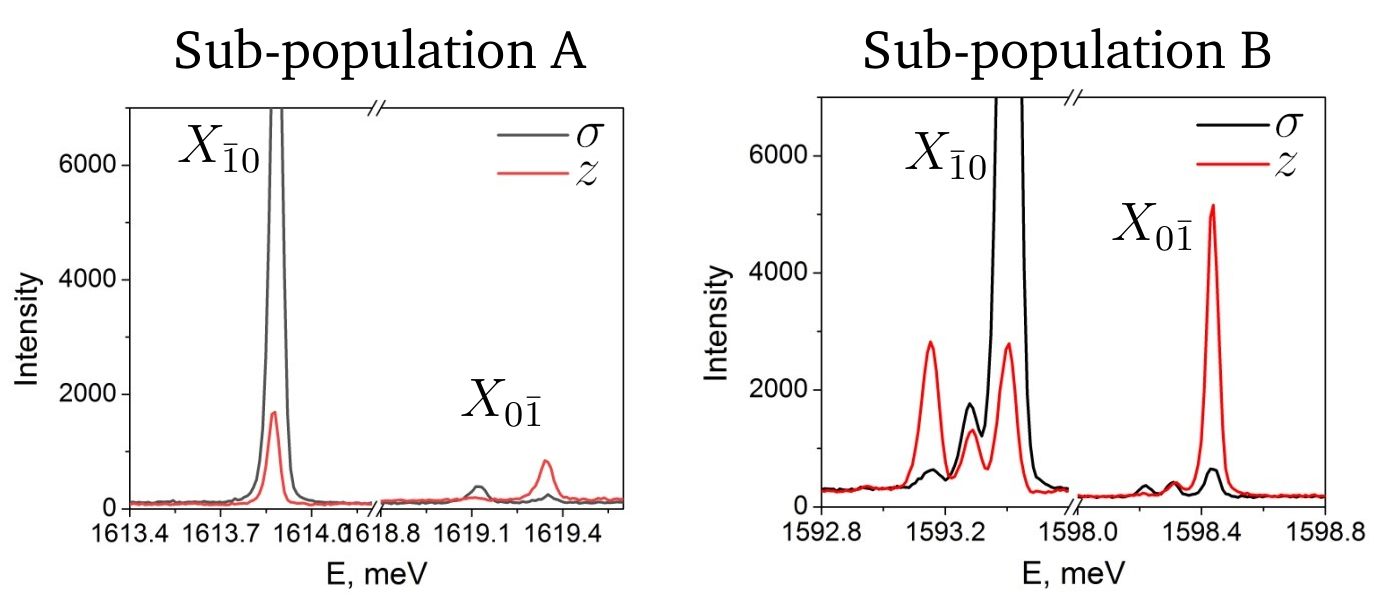
\includegraphics[width=\textwidth]{figures/single_neutral}
\end{center}
\caption{Spectra of two types of QDs in the neutral exciton decays. The $\sigma$ and $z$-polarised spectra are colour-coded black and red, respectively.\label{fig:single_neutral}}
\end{figure}

$$X^-_{\bar{1}0}$$
$$X^-_{0\bar{1}}$$


\section{Discussion of results}

\subsection{Agreement with the bulk symmetry $T_d$}
Observing which exciton complexes seem to elevate to $T_d$ generates predictions within our theory about the localisation of their wavefunctions within the QD bulk. The exciton transitions which were observed to undergo symmetry elevation to $T_d$ in the MCJP dataset are $X_{\bar{1}0}$ (for one sub-population), $X^-_{\bar{1}0}$ (not in the Karlsson data), $2X^+_{\bar{2}1}$ (with one peak being ambiguously identified to belong to the transition), $X^+_{\bar{1}1}$ (for one sub-population),  $X^+_{1\bar{1}}$ (with the relative intensity of the polarisations not explicable with symmetry arguments), and $2X_{\bar{2}0}$ (assuming the $6$ lines are unresolvable due to tight spacing). Conversely, the excitons $X_{0\bar{1}}$ (for one sub-population), $X^+_{\bar{1}1}$ (for one sub-population), and $X^+_{1\bar{1}}$ (only in the Karlsson data) seem to explicitly disconfirm $T_d$ symmetry and probe for the structure symmetry. It is important to note that the sub-population divisions for the neutral excitons and for the positive excitons are different.

It should be noted that transitions for all other exciton complexes measured by Karlsson \textit{et al.} agree with the structure symmetry $C_{3v}$ \cite[p.~20]{karlsson}.

The claim in Sec.~\ref{sec:localisation} is disproven by the transition $X^+_{\bar{2}0}$, which, per Karlsson \textit{et al.}, obeys the structure symmetry, unlike positive excitons with one heavy and one light hole. However, the other exciton complexes with only heavy holes and $1$ or $2$ electrons seem to elevate to the bulk symmetry, hence the exciton localisation may still be the factor determining elevation towards the bulk symmetry, if the delocalisation of $X^+_{\bar{2}0}$ can be justified with a more precise model.

The ambiguity for mixed-hole excitons suggests that light holes indeed may, in general, probe the structure symmetry due to their delocalisation. Neither MCJP not Karlsson \textit{et al.} were able to resolve the light hole-dominant excitons for which the predictions of $C_{3v}$ and $T_d$ differ ($X^+_{0\bar{2}}$, $2X_{0\bar{2}}$, and positive biexcitons with $2$ or $3$ light holes). Resolving these transitions is important material for further study, since if they behave according to structure symmetry, it would be evidence that the symmetry suppression model correctly identifies the mechanism for symmetry elevation.

Regarding the transition $X^+_{1\bar{1}}$ (Fig.~\ref{fig:exciton_positive}), Karlsson \textit{et al.} have experimentally measured the fine-strucure energy splitting of the exciton complex $X^+_{11}$, ordering its corresponding energy levels labelled by their transformation properties \cite[p.~16]{karlsson}. In $C_{3v}$, the lowest and highest energy levels transform as $E_{3/2}$, and the middle two energy levels transform as $E_{1/2}$ \cite[Fig.~17]{karlsson}. This could explain the relative intensities of differently-polarised components of lines in the MCJP dataset, with the $z$-polarisation dominance in lines $c,b$ caused by the different transformation properties of their initial states compared to the initial states of lines $d,a$. It is possible that the wavefunction centre-localisation depends on the exciton transformation properties, affecting the magnitude of symmetry suppression enjoyed only by specific lines within a single exciton transition.

\subsection{Possible sources of error from theoretical treatment and experimental setup}

In our treatment of the exciton envelope functions, we disregard band-mixing effects caused by the nanocrystal structure and small number of lattice points (Sec.~\ref{sec:envelopes}). However, the pyramidal QDs subject to this study exhibit strong valence band mixing, which affects photoluminiscence polarisation \cite{strong_band_mixing}. This may affect the envelope function treatment, especially outside of the $\Gamma$ point, as it contradicts an assumption in the treatment. A more mathematically robust treatment of envelope functions is crucial material for further study.

An important phenomenon disregarded in our treatment is the effect of structure interfaces, which affect the Hamiltonian symmetry group \cite{interfaces}. Whilst a full treatment of the symmetry suppression model has to address this to prove elevation to $T_d$ is still possible, this could also validate our data by providing the polarisation bias to $X^+_{1\bar{1}}$, explaining the relative line intensities.

Finally, for all transitions where we identify elevation to $T_d$, the main evidence consists of the increased number of $z$-polarised lines from the number predicted by $C_{3v}$ and $D_{3h}$. Hence our argumentation relies on the fact that these $z$-polarised components were identified correctly. However, if a physical effect unaccounted for in the experimental setup caused the reading of a non-zero $z$-polarised component where the emission has no $z$-polarised component, the measured $z$-polarised line would match the frequency of the measured $\sigma$-polarised line, analogously to how the non-polarised light predicted by $T_d$ produces lines of matching frequencies in both polarisations. This alternative explanation is supported by the apparent partial disagreement between the MCJP and Karlsson \textit{et al.} datasets specifically regarding the presence of $z$-polarised lines (Fig.~\ref{fig:single_negative},~\ref{fig:biexciton_neutral}). In future study, careful reproduction of the $z$-polarised spectra for exciton complexes identified as elevating to bulk symmetry is crucial for disproving the symmetry suppression hypothesis.

\subsection{Insufficient treatment of line number increase} \label{sec:failed_degeneracy}
The model of symmetry suppression postulates that excitons with wavefunctions localised in the QD bulk enjoy approximate elevation to the bulk (lattice symmetry). Within this model, lines which are light in the lower symmetry but dark in the elevated symmetry will be heavily suppressed. However, the opposite effect (where the number of lines increases with symmetry elevation), which occurs for certain excitons when elevating to $T_d$, is non-trivial to include in the model. This is because the increase of number of lines is often caused by the change of transformation properties of holes when the light hole band and heavy hole band become degenerate at $\Gamma$ (Table~\ref{tab:multihole_states}). Within symmetry suppression theory, we consider the component of a low-symmetry eigenstate which forms an eigenstate of a high-symmetry Hamiltonian, but the residual component still demands different energy levels for the two hole types, suppressing the band distance but keeping it non-zero. For the model to be rigorous, additional treatment of this phenomenon must be introduced, either resolving the transformation properties of holes  under elevation to a group with the hole bands degenerate, or by identifying a mechanism that couples the different-character holes together, salvaging the degenerate behavour within our model. This is material for further study of symmetry elevation within the symmetry suppression framework.

\subsection{Symmetry outside of the $\Gamma$ point} \label{sec:symmetry_outside_gamma}
In the symmetry suppression model, we have assumed all excited fermions to have zero crystal momentum, which is necessary to use the ``charged particles in a box'' dynamics for envelope functions. However, this is only an approximation based on the nature of the direct band-gap of InGaAs. For an excited fermion outside of the $\Gamma$ point in a large crystal, the non-zero crystal momentum vector $\vec{k}$ breaks the wavefunction symmetry, as described by Dresselhaus in \cite[Ch.~13]{dresselhaus}. In an interplay with the bulk symmetry, the true symmetry of the Hamiltonian $\hat{H}\left(\vec{k}\right)$ depends on the crystal momentum. 

In our nanocrystal, the effects of the crystal size alter the band structure, and a full description of the wavefunction is not possible with the crystal momentum, but rather with the shape of the envelope function, which is poorly understood. Exciting the envelope function from the ground state (i.e. leaving the $\Gamma$ point) may break some symmetries, but in general, it also changes the transformation properties of the wavefunction, since $\chi^{\left(\Upsilon\left(\vec{r}\right)\right)}\left(\hat{R}\right)$ in Eq.~(\ref{eq:character_breakdown}) is no longer always unity. This could potentially explain the division of QDs into two sub-populations for some exciton complexes (and the discrepancy with the Karlsson data), where the distribution of envelope function energies would become a non-trivial statistical phenomenon. However, the shapes of the envelope functions are not yet well understood, as they are highly sensitive to high-order or mechanical effects, such as strain-induced piezoelectricity (Fig.~\ref{fig:lens_envelopes}).

Of course, since the extra degree of freedom in transformation properties could alter any prediction for photoluminiscence spectrum, it may also serve as an alternative explanation to symmetry elevation. This is material for further study.\\
\makebox[0pt][l]{%
\begin{minipage}{\textwidth}
\centering
    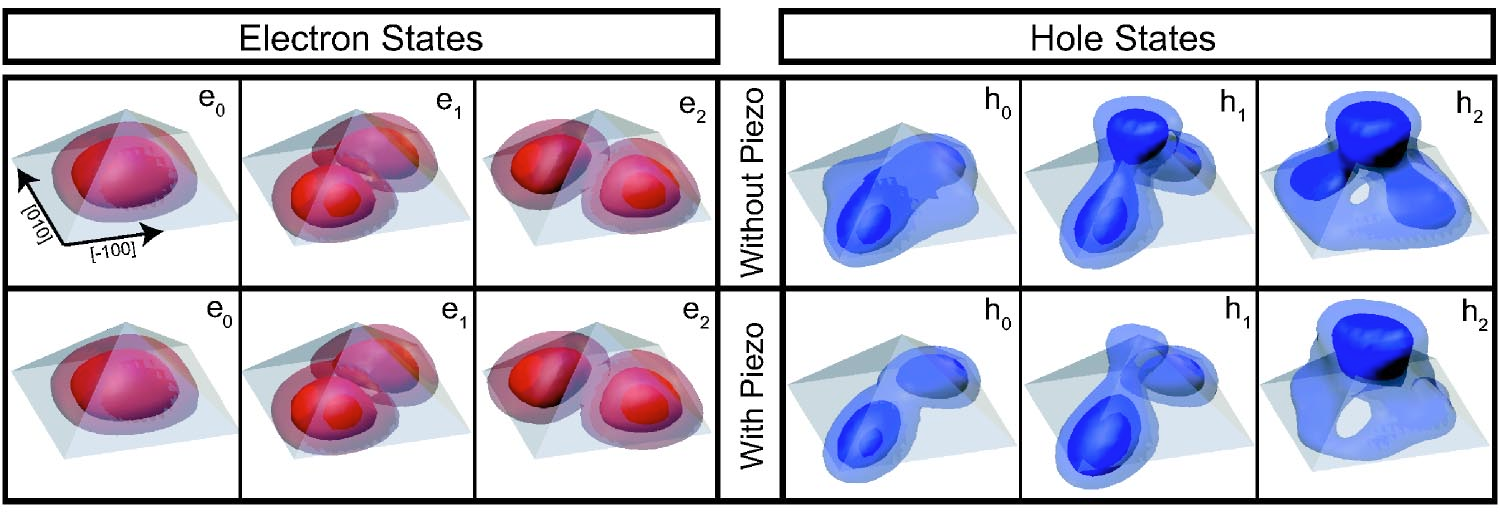
\includegraphics[width=\textwidth]{figures/pyramid_envelopes}
 \captionof{figure}{Envelope functions of ground- and excited-state electrons and holes in a $C_{4v}$ pyramid structure for first-order theory and including strain-induced piezoelectric effect. Figure taken from \cite[Fig.~6]{bulk_limiting}}
 \label{fig:lens_envelopes}
\end{minipage}
}

\chapter{Conclusions} \label{sec:conclusions}

Based on the arguments in \cite{bulk_limiting} and our analysis of the zincblende lattice of InGaAs quantum dots, we claim that neither of the symmetry groups proposed by Karlsson \textit{et al.} ($D_{3h}, C_{6v}$) can be the symmetry group of the Hamiltonian under symmetry elevation. In our model, where the extra symmetries are provided by the atomic lattice in the nanocrystal bulk, we have outlined a general condition for a possible elevated-symmetry group given by the true symmetry and the bulk symmetry (Eq.~(\ref{eq:group_chain})). In general, the true symmetry group $G_s$ may be lower than the structure symmetry due to mismatching orientation of rotations for structure symmetries and bulk symmetries.

Applying this method, we have identified $T_d$ as the only candidate group which $C_{3v}$ can elevate to. Comparing the predictions for emission spectra arising from this group to the to-be published MCJP data, we find partial agreement, suggesting certain excitons undergoing elevation to $T_d$ for at least a certain fraction of the grown QDs.

The true symmetry of the Hamiltonian may be a different subgroup of $T_d$ if prior symmetry breaking occurs in the system, e.g. due to interface effects, piezo-electric or other strain-induced effects, excited-state envelope functions, or other untreated physical phenomenons. Testing the predictions given by subgroups of $T_d$ which do not contain $C_{3v}$ is material for further study, as finding agreement with such a group can also provide clues about the nature of symmetry breaking in the system.

We have constructed a theoretical model of symmetry suppression in Sec.~\ref{sec:symmetry_suppression} as a proposed mechanism for elevating towards bulk symmetry. The model suffices to explain the approximate darkening (suppression) of emission lines as identified by Karlsson \textit{et al.}, but fails to justify the raised degeneracy of valence bands at $\Gamma$ which is required to reach $T_d$ symmetry (Sec.~\ref{sec:failed_degeneracy}). A more robust treatment, possibly incorporating higher-order effects and band-mixing effects is needed to justify this corollary of symmetry elevation to $T_d$.

Within the model of symmetry suppression, excitons are more likely to elevate to bulk symmetry if more of their holes are heavy-like. We conclude that this is untrue for positively charged excitons, but holds for all other exciton and biexciton complexes, hinting at a mechanism affecting wavefunction localisations which is untreated in our simplistic model in Sec.~\ref{sec:localisation}. The exciton transitions $X^+_{0\bar{2}}$, $2X_{0\bar{2}}, 2X^+_{\bar{1}2}, 2X^+_{1\bar{2}}, 2X^+_{0\bar{3}}$ were not yet experimentally resolved, and if future studies demonstrate these transitions to behave according to the structure symmetry, it would both provide evidence that symmetry suppression is the mechanism for symmetry elevation and predict within the model that the associated exciton complexes are not localised in the centre of the quantum dot.

As demonstrated by the discrepancies between the MCJP and Karlsson datasets, as well as the different behaviours of distinct QDs within each dataset, the features of the photoluminiscence spectra of these structures cannot be reliably predicted only by arguments based on the structure and bulk symmetry properties. While a good stepping stone, a fuller understanding of both the symmetry of the true Hamiltonian and other effects which may affect the photoluminiscence spectrum is needed.


\section{Acknowledgements}
The author would like to acknowledge his project partner for his robust, multi-faceted contribution to the project, which includes authoring novel ideas as well as consulting ideas proposed by the author, tirelessly delving into research of countless subjects related to the project, aptly assessing the relevance of the many components of the complex theory of semiconductor nanocrystals to the symmetry properties of quantum dots, diligently validating the outputs of the author's automated algorithm package for double group representation theory with pen-and-paper calculations, identifying many problems and bugs in the process, and many other contributions to the team-work and the team-spirit, from proposing efficient work delegation to engaging in casual conversations about the relationship between mathematics, philosophy, and Nature,

our supervisor, Professor Dimitri Vvedensky, for his guidance, direction, and identification of important information sources, and who supported us throughout the entire duration of the research, discussed the many ideas we proposed to him, and provided invaluable perspective on different aspects of our research when things became overwhelming for us,

Francesco Mattana, Luca Colavecchi, Doctor Gediminas Juska, and Doctor Emanuele Pelucchi from Tyndall National Institute, University College Cork, who kindly provided us with their measurements of the quantum dot photoluminiscence spectra, which constitute material for their to-be-published paper, and with whom we had many stimulating discussions about the quantum dot symmetries,

Professor Jing Zhang, for his consultation on the envelope function method and other fundamental properties of quantum dots,

and Ivan Shalashilin, Jacob Edginton, and the author's family for their discussion and support.

\pagebreak

\section{Bibliography}
\renewcommand\refname{}

\begingroup
\let\clearpage\relax
\vspace{-1cm} % the removed space. Set as appropriate

\begin{thebibliography}{10}

\bibitem{quantum_information1}
Michler, P. (2017), \textit{Quantum Dots for Quantum Information Technologies}. 1st edn. Springer Cham. \href{https://doi.org/10.1007/978-3-319-56378-7}{doi.org/10.1007/978-3-319-56378-7}

\bibitem{quantum_information2}
Juska, G. \textit{et al.} (2016), A Site-Controlled Quantum Dot Light-Emitting Diode of Polarization-Entangled Photons, Violating Bell's Inequality. \textit{CLEO: QELS\_Fundamental Science 2016} (conference). Available at \href{https://opg.optica.org/abstract.cfm?uri=CLEO\_QELS-2016-FTu1C.2}{opg.optica.org/abstract.cfm?uri=CLEO\_QELS-2016-FTu1C.2}

\bibitem{photonics1}
Jin, X. \textit{et al.} (2020), Cation exchange assisted synthesis of ZnCdSe/ZnSe quantum dots with narrow emission line widths and near-unity photoluminescence quantum yields. \textit{Chem. Commun.}, \textbf{56} (45), 6130--6133. \href{https://doi.org/10.1039/D0CC01302A}{doi.org/10.1039/D0CC01302A}

\bibitem{photonics2}
Hanifi, D. A. \textit{et al.} (2019), Redefining near-unity luminescence in quantum dots with photothermal threshold quantum yield. \textit{Science}, \textbf{363} (6432), 1199--1202. \href{https://doi.org/10.1126/science.aat3803}{doi.org/10.1126/science.aat3803}

\bibitem{medicine1}
Medintz, I. L. \textit{et al.} (2005),
Quantum dot bioconjugates for imaging, labelling and sensing. \textit{Nature Mater.}, \textbf{4}, 435--446. \href{https://doi.org/10.1038/nmat1390}{doi.org/10.1038/nmat1390}

\bibitem{medicine2}
Sakimoto, K. K., Wong, A. B., Yang, P. (2016), Self-photosensitization
of nonphotosynthetic bacteria for solar-to-chemical production. \textit{Science}, \textbf{351} (6268), 74--77. \href{https://doi.org/10.1126/science.aad3317}{doi.org/10.1126/science.aad3317}

\bibitem{other_applications}
García de Arquer, F. P. \textit{et al.} (2021), Semiconductor quantum dots: Technological progress and future challenges. \textit{Science}, \textbf{373} (6555). \href{https://doi.org/10.1126/science.aaz8541}{doi.org/10.1126/science.aaz8541}

\bibitem{atomlike}
Ashoori, R. C. (1996), Electrons in artificial atoms. \textit{Nature}, \textbf{379}, 413--419. \href{https://doi.org/10.1038/379413a0}{doi.org/10.1038/379413a0}

\bibitem{tunable}
Cho, A. Y., Arthur, J. R. (1975), Molecular beam epitaxy. \textit{Progress in Solid State Chemistry}, \textbf{10} (3), 157--191. \href{https://doi.org/10.1016/0079-6786(75)90005-9}{doi.org/10.1016/0079-6786(75)90005-9}

\bibitem{karlsson}
Karlsson, K. F. \textit{et al.} (2015), Spectral signatures of high-symmetry quantum dots and effects of symmetry breaking. \textit{New J. Phys.}, \textbf{17}, 103017. \href{https://doi.org/10.1088/1367-2630/17/10/103017}{doi.org/10.1088/1367-2630/17/10/103017}

\bibitem{charge_state}
Hartmann, A. \textit{et al.} (2000), Few-Particle Effects in Semiconductor Quantum Dots: Observation of Multicharged Excitons. \textit{Phys. Rev. Lett.}, \textbf{84} (24), 5648--5651. \href{https://doi.org/10.1103/PhysRevLett.84.5648}{doi.org/10.1103/PhysRevLett.84.5648}

\bibitem{wightman}
Wightman, A. S. (1995), Eugene Paul Wigner 1902--1995. \textit{Notices Amer. Math. Soc.}, \textbf{42} (7), 769-771. Available at \href{https://www.ams.org/notices/199507/wigner.pdf}{www.ams.org/notices/199507/wigner.pdf}

\bibitem{karlsson_2010}
Karlsson, K. F. \textit{et al.} (2010), Fine structure of exciton complexes in high-symmetry quantum dots: Effects of symmetry breaking and symmetry elevation. \textit{Phys. Rev. B}, \textbf{81} (16), 161307(R). \href{https://doi.org/10.1103/PhysRevB.81.161307}{doi.org/10.1103/PhysRevB.81.161307}

\bibitem{dupertuis}
Dupertuis, M. A. \textit{et al.} (2011), Symmetries and the Polarized Optical Spectra of Exciton Complexes in Quantum Dots. \textit{Phys. Rev. Lett.}, \textbf{107} (12), 127403. \href{https://doi.org/10.1103/PhysRevLett.107.127403}{doi.org/10.1103/PhysRevLett.107.127403}

\bibitem{pyramidal_qds}
Hartmann, A. \textit{et al.} (1997), Self-limiting growth of quantum dot heterostructures on nonplanar $\{111\}B$ substrates. \textit{Appl. Phys. Lett.}, \textbf{71} (10), 1314--1316. \href{https://doi.org/10.1063/1.119882}{doi.org/10.1063/1.119882}

\bibitem{hexagon}
Holsgrove, K. M., O'Reilly, T. I., Varo, S. \textit{et al.} (2022), Towards 3D characterisation of site-controlled InGaAs pyramidal QDs at the nanoscale. \textit{J Mater Sci}, \textbf{57} 16383--16396. \href{https://doi.org/10.1007/s10853-022-07654-2}{doi.org/10.1007/s10853-022-07654-2}

\bibitem{semiconductor_handbook}
Goldberg, Y. A., Schmidt, N. M. (1996), \textit{Gallium Indium Arsenide ($\text{Ga}_{x}\text{In}_{1-x}\text{As}$)} in \textit{Handbook Series on Semiconductor Parameters: Volume 2: Ternary And Quaternary III-V Compounds} (edited by Levinshtein, M., Rumyantsev, S., Shur, M.). World Scientific, London. ISBN  981-02-1420-0 (Set)

\bibitem{singh}
Singh, J. (2003), \textit{Electronic and Optoelectronic Properties of Semiconductor Structures} (1st ed.). Cambridge University Press, Cambridge. \href{https://doi.org/10.1017/CBO9780511805745}{doi.org/10.1017/CBO9780511805745}

\bibitem{envelope_fundamentals}
Burt, M. G. (1999), Fundamentals of envelope function theory for electronic states and photonic modes in nanostructures. \textit{J. Phys.: Condens. Matter}, \textbf{11} (9), 53. \href{https://doi.org/10.1088/0953-8984/11/9/002}{doi.org/10.1088/0953-8984/11/9/002}

\bibitem{dresselhaus_condensed_matter}
Dresselhaus, M. S., Dresselhaus, G., Jorio, A. (2007), \textit{Group Theory: Application to the Physics of Condensed Matter} (1st ed.). Springer Berlin, Heidelberg. \href{https://doi.org/10.1007/978-3-540-32899-5}{doi.org/10.1007/978-3-540-32899-5}

\bibitem{envelope_equation}
Burt, M. G. (1992), The justification for applying the effective-mass approximation to microstructures. \textit{J. Phys.: Condens. Matter}, \textbf{4} (32), 6651--6690. \href{https://doi.org/10.1088/0953-8984/4/32/003}{doi.org/10.1088/0953-8984/4/32/003}

\bibitem{dresselhaus}
Dresselhaus, M. S. (2002), \textit{Applications of Group Theory to the Physics of Solids}. Massachusetts Institute of Technology (unpublished). Available at \href{http://web.mit.edu/course/6/6.734j/www/group-full02.pdf}{web.mit.edu/course/6/6.734j/www/group-full02.pdf}

\bibitem{altmann}
Altmann, S. L., Herzig, P. (1994), \textit{Point-Group Theory Tables}. Clarendon Press, Oxford. ISBN 0-19-855226-2

\bibitem{fox}
Fox, M. (2002), \textit{Optical Properties of Solids (Oxford Master Series in Physics)} (1st ed.). Oxford University Press. ISBN 0-19-850613-9

\bibitem{zincblende_symmetry}
Parmenter, R. H. (1955), Symmetry Properties of the Energy Bands of the Zinc Blende Structure. \textit{Phys. Rev.}, \textbf{100} (2), 573--579. \href{https://doi.org/10.1103/PhysRev.100.573}{doi.org/10.1103/PhysRev.100.573}

\bibitem{wigner}
Wigner, E. P. (1959), \textit{Group Theory and Its Application to the Quantum Mechanics of Atomic Spectra} (transl. by Griffin, J. J.) (Expanded and improved ed.). Academic Press, New York and London. Library of Congress Catalog Card No. 59-10741 (Original work published in 1951)

\bibitem{gaas_bonding}
Hsiaw, H. C. \textit{et al.} (1988), Valence and conduction band molecular-orbital topologies and the optical and electrical properties of gallium arsenide and silicon. \textit{J. Non-Cryst. Solids}, \textbf{105} (1--2), 101--106. \href{https://doi.org/10.1016/0022-3093(88)90343-2}{doi.org/10.1016/0022-3093(88)90343-2}

\bibitem{zincblende_lattice_structure}
Tournet, J. (2015), \textit{Growth and Characterization of Epitaxial Al Layers on GaAs and Si Substrates for Superconducting CPW Resonators in Scalable Quantum Computing Systems} (MASc thesis, University of Waterloo). Waterloo, Ontario. Available at \href{https://core.ac.uk/download/pdf/144148499.pdf}{core.ac.uk/download/pdf/144148499.pdf}

\bibitem{landau}
Landau, L. D., Lifshitz, E. M. (1977, repr. 1991 w. corrections), \textit{Quantum Mechanics: Non-Relativistic Theory} (transl. by Sykes, J. B., Bell, J. S.) (3rd ed., revised a. enlarged). Pergamon Press, Oxford. ISBN 0-08-020940-8 (Translated from 4th ed. published in 1989)

\bibitem{bulk_limiting}
Bester, G., Zunger, A. (2005), Cylindrically shaped zinc-blende semiconductor quantum dots do not have cylindrical symmetry: Atomistic symmetry, atomic relaxation, and piezoelectric effects. \textit{Phys. Rev. B}, \textbf{71} (4), 045318. \href{https://doi.org/10.1103/PhysRevB.71.045318}{doi.org/10.1103/PhysRevB.71.045318}

\bibitem{strong_band_mixing}
Zhu, Q. \textit{et al.} (2007), Transition from two-dimensional to three-dimensional quantum confinement in semiconductor quantum wires/quantum dots. \textit{Nano Lett.}, \textbf{7} (8), 2227--33. \href{https://doi.org/10.1021/nl0706650}{doi.org/10.1021/nl0706650}

\bibitem{interfaces}
Tomić, S., Vukmirović, N. (2011), Symmetry reduction in multiband Hamiltonians for semiconductor quantum dots: The role of interfaces and higher energy bands. \textit{J. Appl. Phys.}, \textbf{110} (5), 053710. \href{https://doi.org/10.1063/1.3631048}{doi.org/10.1063/1.3631048}

%\bibitem{biedenharn}
%Biedenharn, L. C., Louck, J. D. (2009), \textit{Angular Momentum in Quantum Physics: Theory and Application (Encyclopedia of Mathematics and its Applications, Series Number 8)} (illustrated ed.). Addison-Wesley Publishing Company, Advanced Book Program. ISBN 0-201-13507-8

\end{thebibliography}


\bibliographystyle{unsrt}
% use the following line to create a bibligraphy based on a .bib bibtex file (change to your filename)
%\bibliography{michal_bibliography}

\endgroup





% that's all folks
\end{document}


